\documentclass{article}
\usepackage{graphicx} 
\usepackage{float}
\usepackage{booktabs}
\usepackage{array}
\usepackage{arydshln}
\usepackage{siunitx}
\usepackage{hyperref}
\usepackage{cancel}
\usepackage{changepage}
\usepackage{placeins}
\usepackage{enumitem}

%\usepackage{showframe}
%\usepackage{times}

\usepackage{tabularx}
\usepackage{amsmath, amssymb, amscd, MnSymbol, mathrsfs}
\usepackage{cellspace}
\usepackage{tikz}
\usetikzlibrary{calc, patterns, angles, quotes, decorations.markings, decorations.pathmorphing, hobby}
\usepackage{xfrac}

\usepackage{chemfig}
\usepackage{caption}
\usepackage{tcolorbox}
\usepackage{bm}
\usepackage{pdfpages}
\usepackage{empheq}
\usepackage{pgfplots}
\pgfplotsset{compat=1.18}
\usepackage[oldvoltagedirection]{circuitikz}
\usepackage{microtype}
\usepackage{tikz-3dplot}
\usepackage{bibref}
\usepackage{textcomp}
% Custom commands
\newcommand{\vect}[1]{\boldsymbol{\mathbf{#1}}}
\newcolumntype{C}{>{\centering\arraybackslash}X}
\newcolumntype{M}[1]{>{\centering\arraybackslash}m{#1}}

\usetikzlibrary{external}
\tikzexternalize[prefix=figures/]

\newcommand\myfrac[2]{\sfrac{#1\mkern-1.2mu}{#2}}
\usepackage{xcolor}

% Define custom colors
\definecolor{darkblue}{rgb}{0.1,0.1,0.5} % A dark blue shade
\definecolor{formalshade}{rgb}{0.95,0.95,1} % A light blue shade for the background

% For the adjustwidth environment
\PassOptionsToPackage{strict}{changepage}
\usepackage{changepage}

% For formal definitions
\usepackage{framed}

\newcommand{\formalsource}{} % Initialize an empty macro to store the source text

\newenvironment{formal}[1][]{% Start of the environment
    \renewcommand{\formalsource}{#1}% Store the optional argument
    \def\FrameCommand{%
        \hspace{1pt}%
        {\color{darkblue}\vrule width 2pt}%
        {\color{formalshade}\vrule width 4pt}%
        \colorbox{formalshade}%
    }%
    \MakeFramed{\advance\hsize-\width\FrameRestore}%
    \noindent\hspace{-4.55pt}% Disable indenting the first paragraph
    \begin{adjustwidth}{}{7pt}%
        \vspace{2pt}%
    }%
    {%
        \vspace{4pt}%
        \ifx\formalsource\empty % Check if the source is empty
        \else
        \hfill{\footnotesize{\formalsource}}% Align source to the bottom-right
        \fi
    \end{adjustwidth}\endMakeFramed%
}


% Custom itemize list with images for positive and negative items
\newlist{gitemize}{itemize}{1} % Just one level for the list
\setlist[gitemize,1]{
    leftmargin=2.8em, % Adjust the margin for the list
    labelsep=1em % Control the space between the label and the list item
}

% Define checkmark and cross symbols for positive and negative items
\newcommand{\checkitem}{\raisebox{-0.25\height}{\includegraphics[width=0.4cm]{checkmark.png}}}
\newcommand{\crossitem}{\raisebox{-0.25\height}{\includegraphics[width=0.4cm]{cross.png}}}


\usepackage[margin=1in, left=0.8in, right=0.8in, includeheadfoot]{geometry}
\usepackage{fancyhdr}
\usepackage{graphicx}
\usepackage{tabularray}
\usepackage{varwidth} 


\pagestyle{fancy}
\fancyhf{}


\renewcommand{\headrulewidth}{0.4pt}
\renewcommand{\footrulewidth}{0.4pt}

\fancyhead[L]{
\includegraphics[height=1.2cm]{images/Kingston_University_London_logo_200-tablet.png}}
\fancyhead[R]{EG4019 - ME - Engineering Mechanics and Materials}
\fancyfoot[C]{Department of Mechanical Engineering}
\fancyfoot[R]{\thepage}

\geometry{top=0.5in,bottom=0.69in}
\usepackage{scalerel}

\setlength{\headheight}{30pt}
\setlength{\footskip}{20pt}


\usepackage[export]{adjustbox}
\usepackage{tocloft}
\renewcommand{\cfttoctitlefont}{}
\renewcommand{\contentsname}{}
\renewcommand{\cftsecleader}{\cftdotfill{\cftdotsep}}

\setlength{\cftbeforesecskip}{0.5em}


\usepackage{xurl}

\renewcommand{\theequation}{\text{Eq.}~\arabic{equation}}
%Refer to the equation as \eqref{equation}.
\usepackage{caption}  % This package allows captioning outside of a float
\usepackage[export]{adjustbox}


\usetikzlibrary{patterns}

\usetikzlibrary{patterns.meta}

\pgfdeclarepattern{
    name=hatch,
    parameters={\hatchsize,\hatchangle,\hatchlinewidth},
    bottom left={\pgfpoint{-.1pt}{-.1pt}},
    top right={\pgfpoint{\hatchsize+.1pt}{\hatchsize+.1pt}},
    tile size={\pgfpoint{\hatchsize}{\hatchsize}},
    tile transformation={\pgftransformrotate{\hatchangle}},
    code={
        \pgfsetlinewidth{\hatchlinewidth}
        \pgfpathmoveto{\pgfpoint{-.1pt}{-.1pt}}
        \pgfpathlineto{\pgfpoint{\hatchsize+.1pt}{\hatchsize+.1pt}}
        \pgfpathmoveto{\pgfpoint{-.1pt}{\hatchsize+.1pt}}
        \pgfpathlineto{\pgfpoint{\hatchsize+.1pt}{-.1pt}}
        \pgfusepath{stroke}
    }
}

\tikzset{
    hatch size/.store in=\hatchsize,
    hatch angle/.store in=\hatchangle,
    hatch line width/.store in=\hatchlinewidth,
    hatch size=5pt,           % Smaller hatch size for fewer lines
    hatch angle=45pt,         % More angle to spread lines
    hatch line width=.5pt,    % Thin lines
}

\usepackage[para]{footmisc} % Example of making footnotes run together in a paragraph



\begin{document}
        

    \vspace*{\fill}
    \begin{center}
        \textbf{\Huge Laboratory Report}\\[10pt]
        \LARGE \textbf{Tensile Test}
    \end{center}
    \vspace*{\fill}

    \Large    
    \begin{tabular}{@{}l l l@{}}
        \textbf{Submitted by:} & Sakariye Abiikar (Group Leader)\phantom{ssssss} & K2371673 \\
        & Sandeep Singh & K2314795 \\
        & Aland Floyd Noronha & K2423819 \\
        & Alan Roy & K2314478 \\
        & Judas Surname & K5671234 \\
    \end{tabular}
    
    \vspace*{\fill}
    
    \begin{tabular}{@{}l l@{}}
        \textbf{Key Dates:} & Date of practical: \\
        & Deadline: 31/12/2024 \\
        & Date of submission: \\
    \end{tabular}
    \vspace*{\fill}
    
    \large
    \newpage\noindent\vspace{2em}
    \begin{center}
        \LARGE \textbf{Contribution Table}\\[3em]
    \end{center}
    

    
    \begin{tblr}{
            colspec={Q[4cm]Q[4cm]Q[4cm]Q[3cm]},
            hlines,vlines,
            cells={valign=m,halign=c},
            rows={ht=4\baselineskip},
            row{1}={ht=1.5\baselineskip,font=\bfseries},
        }
        Student & Course & Contribution & Picture \\ 
        Sakariye Abiikar & Mechanical Engineering & Results, Theory, Recommendations & 
\includegraphics[width=2cm,valign=c]{images/profile.jpg} \\ 
        Andrew Surname & Aviation & Introduction & 
\includegraphics[width=2cm,valign=c]{images/profile.jpg} \\ 
        Lucas Surname & Astro & Results & 
\includegraphics[width=2cm,valign=c]{images/profile.jpg} \\ 
        James Surname & Mechanical Engineering & Discussion, References & 
\includegraphics[width=2cm,valign=c]{images/profile.jpg} \\ 
        Judas Surname & Civil Engineering &  & 
\includegraphics[width=2cm,valign=c]{images/profile.jpg} \\ 
    \end{tblr}
    
    \normalsize
    \newpage\noindent\vspace{1em}
    \begin{center}
        \LARGE \textbf{Table of Contents}\\[1.5em]
    \end{center}
    \tableofcontents
    \thispagestyle{fancy}


    \large\newpage\vspace*{-20pt}

    \section{Abstract}
    \vspace*{1em}
    This study investigated the effects of two thermal treatments on the mechanical properties of HE30/BS1476 aluminium alloy, initially characterized by a hardness of 120 HV5, an elastic modulus of 6 GPa, and an ultimate tensile strength of 500 MPa. The alloy underwent two heat treatments: first, heating for 90 minutes at 520\textdegree C, followed by an additional 40 minutes at 184\textdegree C in open air. Three distinct alloy variations were produced as a result of these treatments. The aim of the research was to quantify changes in hardness, modulus of elasticity, yield strength, ultimate tensile strength (UTS), and percentage elongation. Hardness was measured using a Zwick Roell ZHU hardness testing machine with a 5 kg load (HV5) (See Appendix A), and properties such as stress and strain were derived from data obtained using a Zwick Roell 2050 tensile testing machine.
%   {Needs small info on results and reflection/conclusion (to be added at a later date)}
   
    
    \newpage\vspace*{-20pt}
\section{Introduction}

In engineering, the selection and optimization of materials significantly influence the performance of designs, particularly in the aerospace, automotive, and construction industries. Aluminium alloys are highly valued in these sectors due to their excellent strength-to-weight ratio and corrosion resistance, especially in applications requiring mechanical improvements through controlled processes (thyssenkrupp, 2023).\\[8pt]
Research by metallurgists such as Sorby and Sauveur has demonstrated that \textbf{heat treatment} can significantly enhance the properties of alloys. By altering the microstructure, heat treatments improve tensile strength, hardness, and elasticity. Techniques such as quenching and solution heat treatment are tailored to achieve specific mechanical properties based on the alloy’s intended application (Eurotherm, 2024).\\[8pt] 
\textbf{Aging} is a heat treatment process used to enhance the mechanical properties of aluminum alloys. It involves two main stages: first, the alloy is heated to dissolve alloying elements and then rapidly cooled, creating a supersaturated solid solution. Following this, the alloy undergoes artificial aging, where it is reheated to a lower temperature for a set period. This allows for the formation of fine particles that strengthen the material by impeding dislocation movement, thereby improving its hardness and tensile strength. Aging is crucial for optimizing the performance of aluminum alloys used in various applications (Rajaa et al., 2018).\\[8pt]
The significance of heat treatments is further supported by research. In one study, for example, the hardness of Al 6082 alloy increased from 65 BHN to 102 BHN after 8 hours of solution heat treatment. Furthermore, the alloy's tensile strength increased from 154 MPa to 280 MPa after being aged for 6 hours at 205\textdegree C and 495\textdegree C (Singh et al., 2023). Aluminium alloys like HE30 are ideal for demanding applications in the automotive and aerospace industries because of these microstructural improvements.\\[8pt]
This research investigates the response of HE30 aluminium alloy to thermal treatments, focusing on changes in its mechanical properties.

\newpage\vspace*{-20pt}
\section{Method}
This laboratory research primarily focused on evaluating the mechanical properties of our alloy samples, including key metrics such as yield strength, ultimate tensile strength (UTS), modulus of elasticity, hardness, and percentage elongation. These properties are essential for understanding the material's behavior under stress and assessing its suitability for various engineering applications.\\[8pt]
The methodologies employed in this study were designed to optimize the data obtained from individual experiments on the alloys. By utilizing advanced data analysis techniques such as \textbf{Response Surface Methodology (RSM) and Fraction Factorial Design (FFD)} (See Appendix C), we uncovered correlations and dependencies that might otherwise remain hidden. For instance, tensile testing, beyond yielding basic parameters like UTS and modulus of elasticity, provided insights into failure mechanisms and material behavior under specific conditions. This approach reduces the need for extensive experimental operations while deepening our understanding of the alloys' properties and enabling predictive modeling. By focusing on a minimal set of tests that deliver insights into multiple material properties, the methodology ensures each procedure is maximally informative, minimizing resource usage and reducing the likelihood of error.\\[8pt]
Building on this optimized experimental design, the research approach utilized in this study incorporates an \textbf{Integrated Testing Strategy (ITS)}. ITS combines collected data to provide a comprehensive and precise assessment of the alloy's mechanical properties. It reduces redundancy and streamlines the evaluation process by avoiding reliance on a single test or series of tests. As an example of broader interdisciplinary efforts, the ITS developed in this study was designed to reduce operational costs, minimize resource consumption, and shorten the time required to carry out processes (Rovida et al., 2015; Alan Turing Institute, 2024)\\[8pt]
Our approach was characterized by the following key procedures:
\begin{enumerate}[itemsep=-0.5mm]
    \item Dimensional Analysis
    \item Hardness Testing
    \item Tensile Testing 
    \item Data Analysis
\end{enumerate}
\footnote{Note that \textbf{Sample Preparation} is separate from the testing process and is not included as part of the testing itself; therefore, it is not considered a part of the list of procedures in the experiment we conducted.} By designing the experiment with this set of procedures, each offering multiple insights through its respective process, we were able to perform a comprehensive evaluation of the alloy's mechanical properties. This approach minimized time, resource consumption and potential errors, ensuring the accuracy and reliability of the results while providing a robust dataset for detailed analysis and interpretation of the alloy's performance characteristics.

\newpage

\section{Experimental Procedures}
The alloys employed in this study originate from HE30/BS1476. The designation HE30 pertains to a temper classification established under the now-defunct BS 1476 standard, which detailed the heat treatment and aging protocols for aluminium alloys. Introduced in 1955 and revised until 1987, BS 1476 was formally withdrawn on June 21, 2022.\\[8pt]
Despite the withdrawal of BS 1476, the temper designation HE30 remains intrinsically linked to the aluminium alloy 6082, a material extensively utilized in engineering applications. Although the precise parameters defined by BS 1476 are no longer accessible, HE30 is consistently correlated with 6082 and its well-documented temper conditions:
\begin{itemize}[itemsep=1pt]
    \item \textbf{T6}: Solution heat-treated and artificially aged.
    \item \textbf{O}: Fully annealed (softened state).
    \item \textbf{T4}: Solution heat-treated and naturally aged.
    \item \textbf{T651}: Solution heat-treated, stress-relieved, and artificially aged.
\end{itemize}
The absence of BS 1476 does not hinder the characterization of HE30, as the chemical composition of 6082 is standardized under EN 573-3, which aligns with internationally recognized specifications for this alloy. While BS 1476 specifies HE30, BS EN 573-3 defines 6082-T6, ensuring continuity in the alloy's description and application (Acton Bright Steel, 2024).

\subsection{Description}
Key details are as follows:
\begin{formal}[Truventor, 2019]
Aluminium HE 30 alloy a.k.a AL 6082 is a medium strength alloy with excellent corrosion resistance. It has the highest strength of 6000 (6XXX) series alloys. It is also known as a structural alloy. In block, plate, or bar form, AL HE 30 alloy is most commonly used in machining.\\[8pt]
Although it is a relatively new alloy, due to its higher strength, AL HE 30 has replaced AL 6061 in many applications. The addition of a large amount of manganese controls the grain structure which in turn results in a stronger alloy.\\[8pt]
\begin{minipage}[t]{0.57\textwidth}
    \textbf{Characteristics:}
    \begin{itemize}[itemsep=-1mm]
    \item High strength-to-weight ratio makes it ideal for lightweight structures.
    \item Most versatile and highest strength alloy in the 6000 series Aluminum.
    \item Good machinability compared to metals like Stainless Steel (SS) and Mild Steel (MS).
    \item Lightweight and corrosion-resistant components.
    \item Alternative to plastics in high-stress applications.
    \item Lower fatigue strength and elastic strength compared to steels.
\end{itemize}
\end{minipage}\hspace{2.4em}
\begin{minipage}[t]{0.45\textwidth}
\textbf{Applications:}
\begin{itemize}[itemsep=-1mm]
    \item Automotive components.
    \item Electronic applications.
    \item Aerospace components.
    \item Trusses, frames, and beams.
\end{itemize}
\end{minipage}\\
\vspace{1pt}
\end{formal}
\newpage\noindent
Aluminium alloy 6082 and HE30 are corresponding designations, though not precisely equivalent, with minor differences in composition and performance (aalco, 2019). As BS 1476, which defines HE30, was withdrawn in 2022, obtaining its exact specifications would require consulting the British Standards Institution (BSI). For this study, we will treat HE30 as equivalent to 6082, simplifying the analysis of the alloy's properties and subsequent discussions, while acknowledging potential slight differences.
\subsection{Composition}
\centering
\begin{minipage}{0.44\textwidth}
    \centering
    \renewcommand{\arraystretch}{1.4}

        \begin{tabular}{|>{\normalsize\bfseries}l|>{\normalsize}c|}
            \hline
            \large \textbf{Chemical Element} & \textbf{\% Present} \\ \hline
            Aluminium (Al)            & Balance             \\ \hline
            Copper (Cu)               & 0.1 max        \\ \hline
            Magnesium (Mg)            & 0.6 - 1.2         \\ \hline
            Silicon (Si)              & 0.7 - 1.3         \\ \hline
            Iron (Fe)                 & 0.5 max         \\ \hline
            Manganese (Mn)            & 0.4 - 1         \\ \hline
            Zinc (Zn)                 & 0.2 max        \\ \hline
            Chromium (Cr)             & 0.25 max        \\ \hline
            Titanium (Ti)             & 0.1 max        \\ \hline
            Other (Each)              & 0.05 max        \\ \hline
            Others (Total)            & 0.15 max        \\ \hline
        \end{tabular}
        \captionof{table}{Chemical Composition of Alloy 6082 (BS EN 573-3:2009) (aalco, 2019)}
        \label{tab:composition_6082}

        
    \vspace{1em}
    \begin{tabular}{|>{\normalsize\bfseries}l|>{\normalsize}c|}
        \hline
        \large\textbf{Chemical Element} & \large\textbf{\% Present} \\ \hline
        Aluminium (Al)            & Remainder         \\ \hline
        Copper (Cu)               & 0.1 max           \\ \hline
        Magnesium (Mg)            & 0.4 - 1.5         \\ \hline
        Silicon (Si)              & 0.6 - 1.3         \\ \hline
        Iron (Fe)                 & 0.6 max           \\ \hline
        Manganese (Mn)            & 0.4 - 1         \\ \hline
        Zinc (Zn)                 & 0.1 max           \\ \hline
        Chromium (Cr)             & 0.5 max           \\ \hline
        Titanium (Ti)             & 0.2 max           \\ \hline
    \end{tabular}
    \captionof{table}{Chemical Composition of HE30/BS1476 according to Dr. Santiago's Data}
    \label{tab:composition_he30}
\end{minipage}
\hfill
\begin{minipage}{0.53\textwidth}
    The composition of 6082 conforms to the standard specifications for this aluminium alloy at the BS EN 573-3:2009, as detailed in Table \ref{tab:composition_6082}. These values are consistent with industry standards for 6082, providing a foundation for further analysis.\\[8pt]
    Once again, I stress that there may be minor differences in the composition of HE30, especially in accordance with the BS 1476 specifications.\\[8pt] 
    The values listed here are provided for reference, but the exact composition of the specifci HE30 alloy we used should be verified for accurate work in our lab, as it may not align with typical web standards.
    \vspace{1em}\hrule\vspace{1em}
    Although I do have actual information regarding the "Aluminium alloy to the HE30 BS1476 specification" from Dr. Santiago shown in Table \ref{tab:composition_he30}, it is important to note that this source lacks proper documentation, and its credibility remains uncertain.\\[8pt]
    The BS1476 has been withdrawn and has not been explicitly updated or replaced, as I stated. It is still largely unreferenced and not widely recognised in the contemporary literature. So this data provided contradicts to much of what is being currently pertaining to the standard.\\[8pt]
    Although there are significant differences between the two sources in terms of composition, I have chosen to adopt Dr. Santiago's version for the purpose of this work. This decision is based on the fact that the table he provided reflects the information he, as my instructor, has shared with me. While I acknowledge the discrepancies and the lack of clear sourcing in his data, I consider it appropriate to proceed with his version for expediency, particularly as it aligns with the guidance he has given in our coursework.
\end{minipage}\\

\raggedright

\subsection{Heat Treatments and Alloy Conditions}
Each sample was treated under different conditions to evaluate the effect of heat treatment on its mechanical properties. The samples were provided in the typical bone-shaped form for tensile testing. The heat treatment conditions are as follows:
\begin{itemize}[itemsep=-1mm]
    \item \textbf{AR (As Received)}: The sample was used without any heat treatment, in its initial state as supplied.
    
    \item \textbf{ST (Solution Treatment)}: The sample was heated at 520\textdegree C for 90 minutes to dissolve precipitates, improving ductility. The exact quenching method is unspecified.
    
    \item \textbf{PH (Precipitation Hardening)}: The sample was first heated at 520\textdegree C for 90 minutes, followed by aging at 184\textdegree C for 40 minutes to enhance strength and hardness.
\end{itemize}
These treatments were applied to assess how they influence the alloy's mechanical properties.



% Here is the guidline/rules for this subsection
% Experimental procedures describe the precise, step-by-step actions required to carry out an experiment—such as specific instructions like "do this" or "do that"—ensuring repeatability and accuracy in obtaining results. These procedures are intended to allow any individual to physically replicate the experiment.

%SAMPLES: 
% Description of the alloy, Composition, CSA (mention dimensions are measured by a calliper), Nomenclature, Heat treatments, Picture before testing, etc

% HARDNESS: 
% Testing machine (pics), Procedure (pics)

% TENSILE TEST: 
% Machine (pics), Procedure (pics)


\def\imas{2.4cm}
\subsection{Equipment List}
\begin{table}[H]
    \centering
    \begin{tblr}{
            colspec = {Q[4cm] Q[4cm] Q[8cm]},
            hlines, vlines,
            rows={ht=4\baselineskip},
            cell{1-4,6}{1} = {font=\bfseries},
            cells = {valign=m,halign=c},
            column{3} = {valign=h,halign=l},
            row{1} = {ht=2\baselineskip,font=\bfseries,c,m},
        }
        \textbf{Equipment} & \textbf{Image} & \textbf{Reasoning} \\ 
        Digital Caliper & 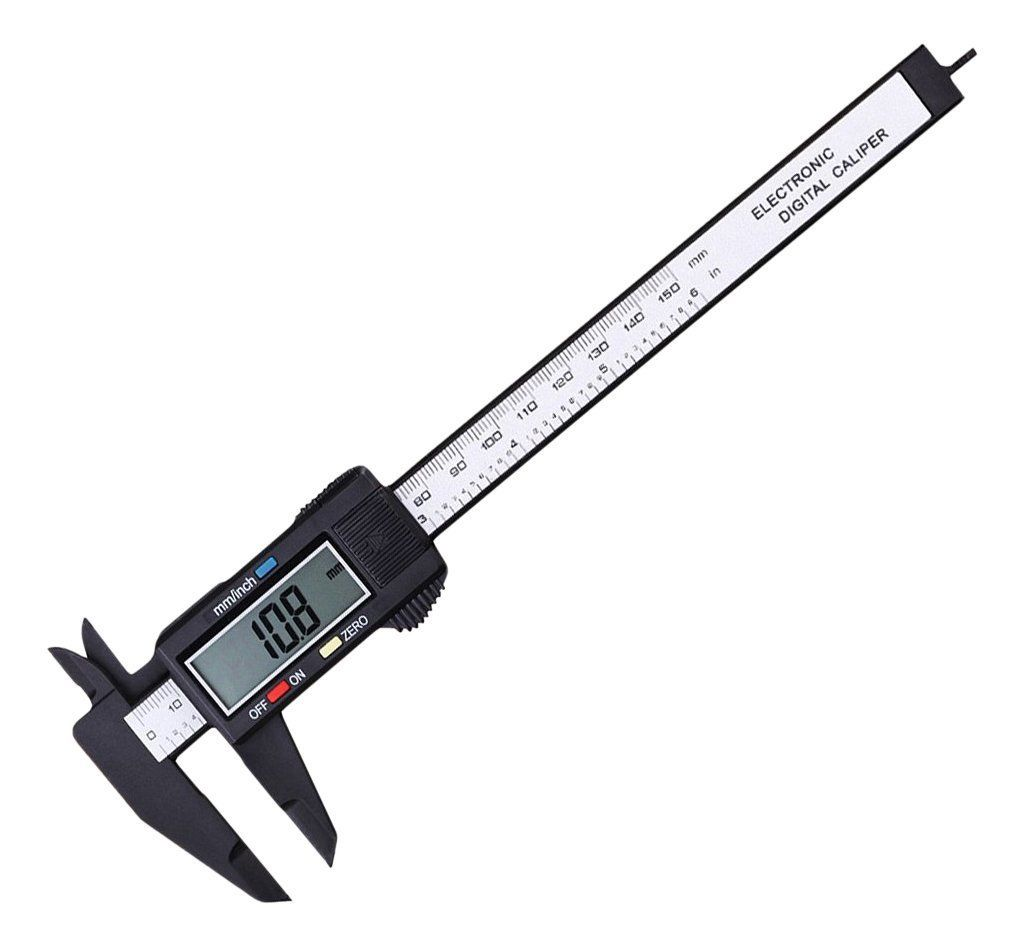
\includegraphics[width=\imas,valign=c]{images/digital_vernier_caliper.jpg} & Enables precise and accurate measurement of small dimensions, such as the diameter, thickness, and depth of samples, crucial for ensuring consistency in experimental setup and results. \\
        Vickers Hardness Testing Machine & 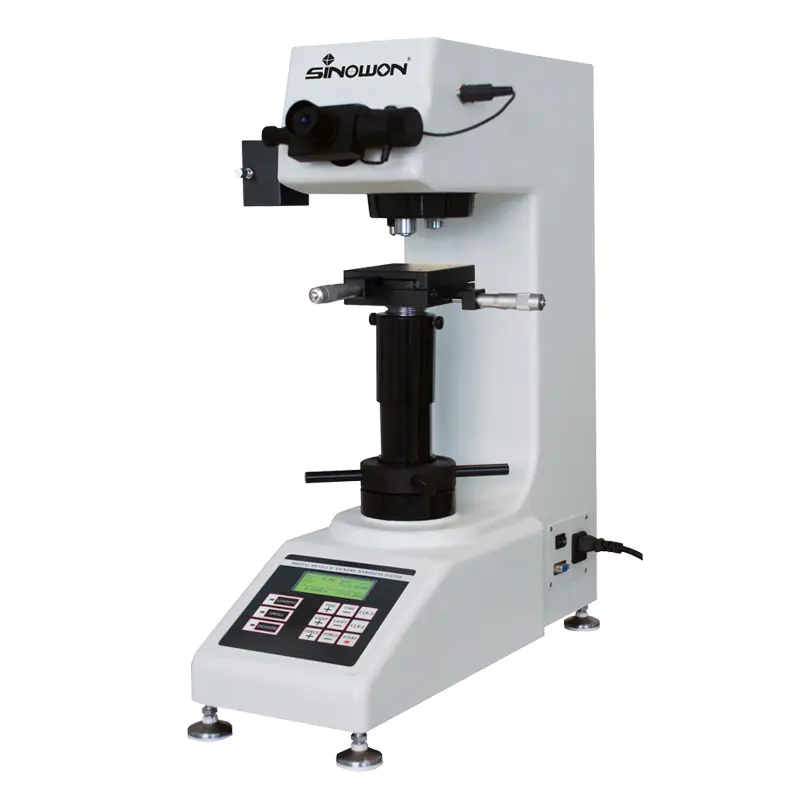
\includegraphics[width=2.1cm,height=2.4cm,valign=c]{images/hardness.png} & Used to assess the hardness of materials by applying a standardized force to create an indentation, which is then measured to determine the material's resistance to deformation. \\
        Zwick Roell 2050 Tensile Testing Machine & 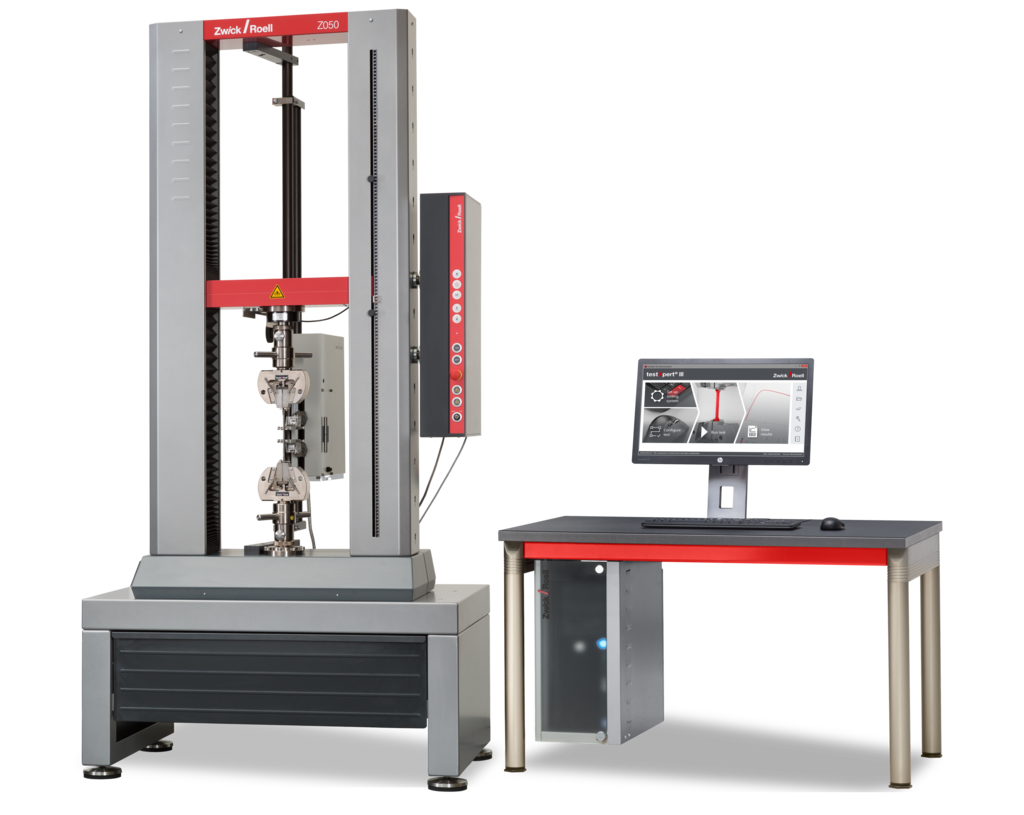
\includegraphics[width=\imas,valign=c]{images/tensilemachine.png} & Evaluates the tensile strength and mechanical properties of materials under uniaxial tension, providing data essential for material performance analysis and comparison. \\
        \textbf{Personal Protective Equipment (PPE):} Safety glasses, closed-toe shoes, lab coat & 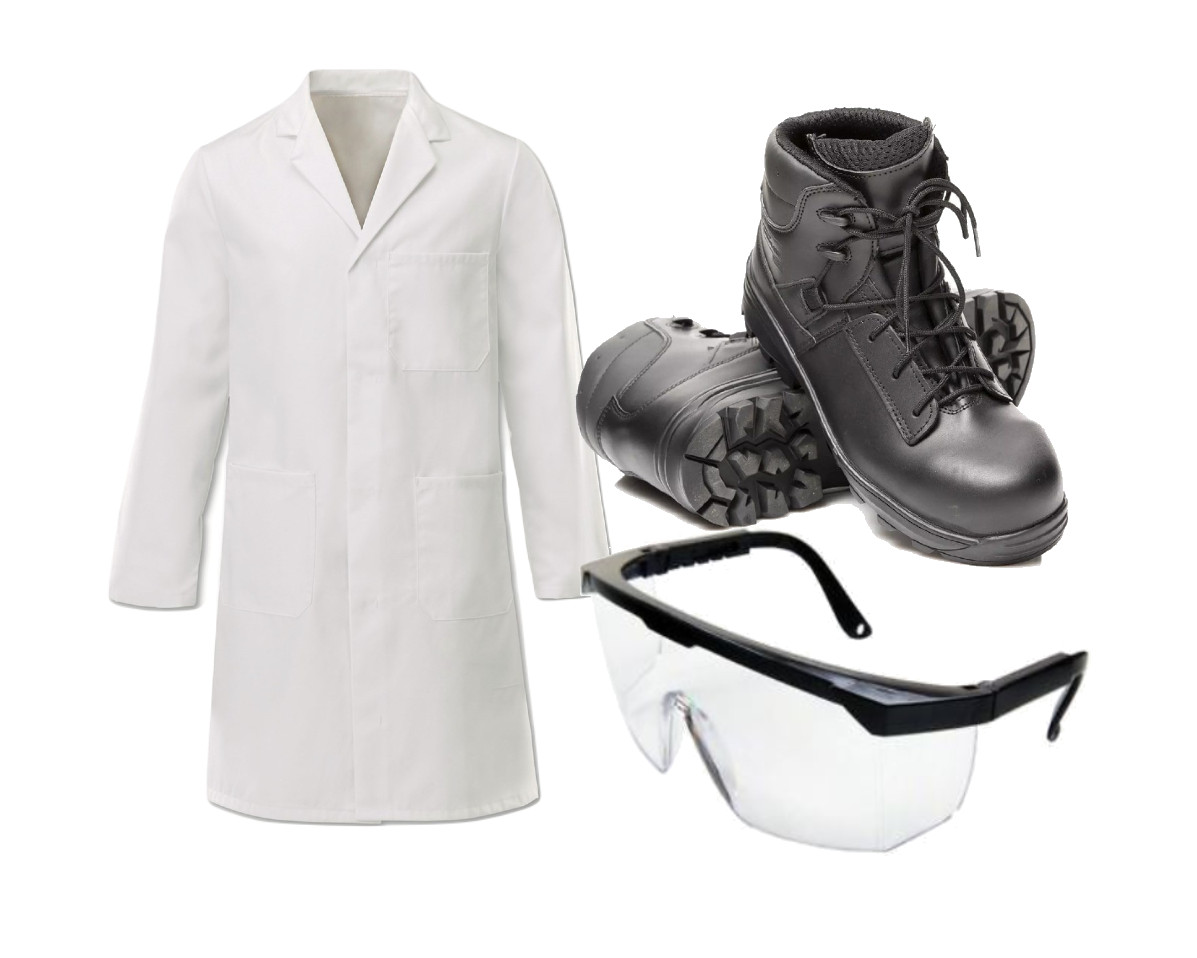
\includegraphics[width=\imas,valign=c]{images/ppe.jpg} & Protects against potential hazards in tensile testing, such as flying debris from specimen fracture, pinch points in the testing machine, and general laboratory risks further shown in Table \ref{tab:risk-assessment}.\\
        Camera/Smartphone and Stationery & 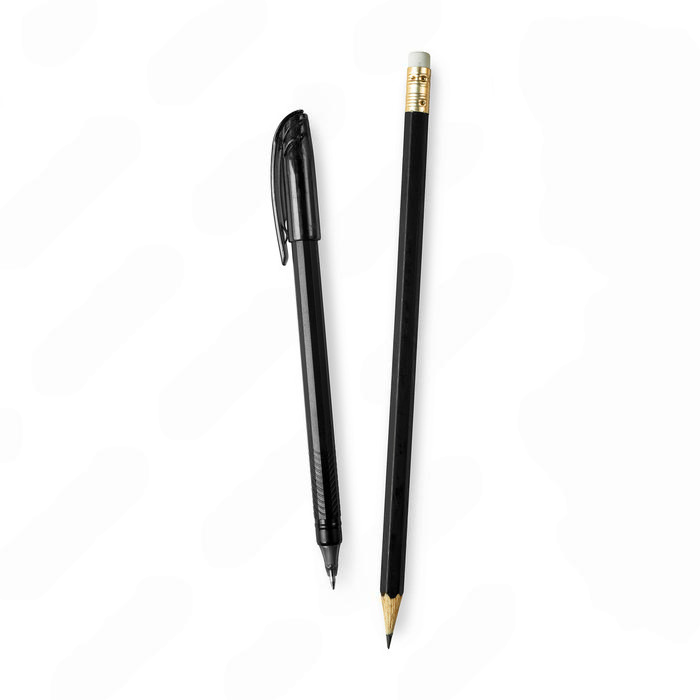
\includegraphics[width=\imas,valign=c]{images/stationary.png} & For documenting experimental setups and procedures, capturing visual evidence of results, and recording detailed observations, calculations, and procedural notes for accurate reporting. \\
    \end{tblr}
    \caption{Overview of Equipment Used in the Experiment}
    \label{tab:equipment_overview}
\end{table}

    

\newcommand{\mr}[2]{%
    \begin{varwidth}{#2}%
        #1%
    \end{varwidth}%
}


\subsection{Risk Assessment}
The experimental procedures involved several potential hazards. The identified risks, their levels, and mitigation strategies are outlined below:
\begin{table}[h!]
    \centering
    \begin{tblr}{
            width=\linewidth,
            colspec={Q[4cm]Q[5cm]Q[2cm,c,m]Q[5cm]},
            rows = {ht=4\baselineskip},
            row{1} = {font=\bfseries,c,m,ht=1.5\baselineskip},            
            rows,columns = {valign=m},
            hlines, vlines
        }
        Hazard & Risk & Level of Risk & Control Measures \\
        Tensile testing machine & \mr{Pinching or crushing injuries from moving parts}{5cm} & High & Keep hands and body away from moving components during operation; follow machine's safety protocols. \\
        \mr{Sharp edges of dogbone samples}{4cm} & \mr{Cuts or injuries while handling samples}{5cm} & Medium & \mr{Handle with care; use gloves when measuring and mounting samples.}{5cm} \\
        \mr{Vickers hardness testing machine}{4cm} & Injury from improper handling or sample misplacement & Medium & Ensure proper training before operation; position samples correctly and keep fingers clear. \\
        \mr{General laboratory environment}{4cm} & Slips, trips, and falls due to clutter or spills & Low & Maintain a tidy workspace; clean spills immediately; wear appropriate footwear. \\
    \end{tblr}
    \caption{Identified hazards, associated risks, levels, and control measures.}
    \label{tab:risk-assessment}
\end{table}

\section{Conducting the Experiment}
For the experiment, we were provided with three samples, which are visually represented in the image below:
\begin{figure}[H] 
    \centering 
    \includegraphics[width=0.6\textwidth,height=0.3\textheight]{example-image} 
    \caption{Visual representation of the three samples} 
    \label{fig:samples} 
\end{figure}
\newpage\noindent
Additionally, we were given an A4 sheet with a form to complete, which looked as shown below:

\begin{figure}[H] 
    \centering 
    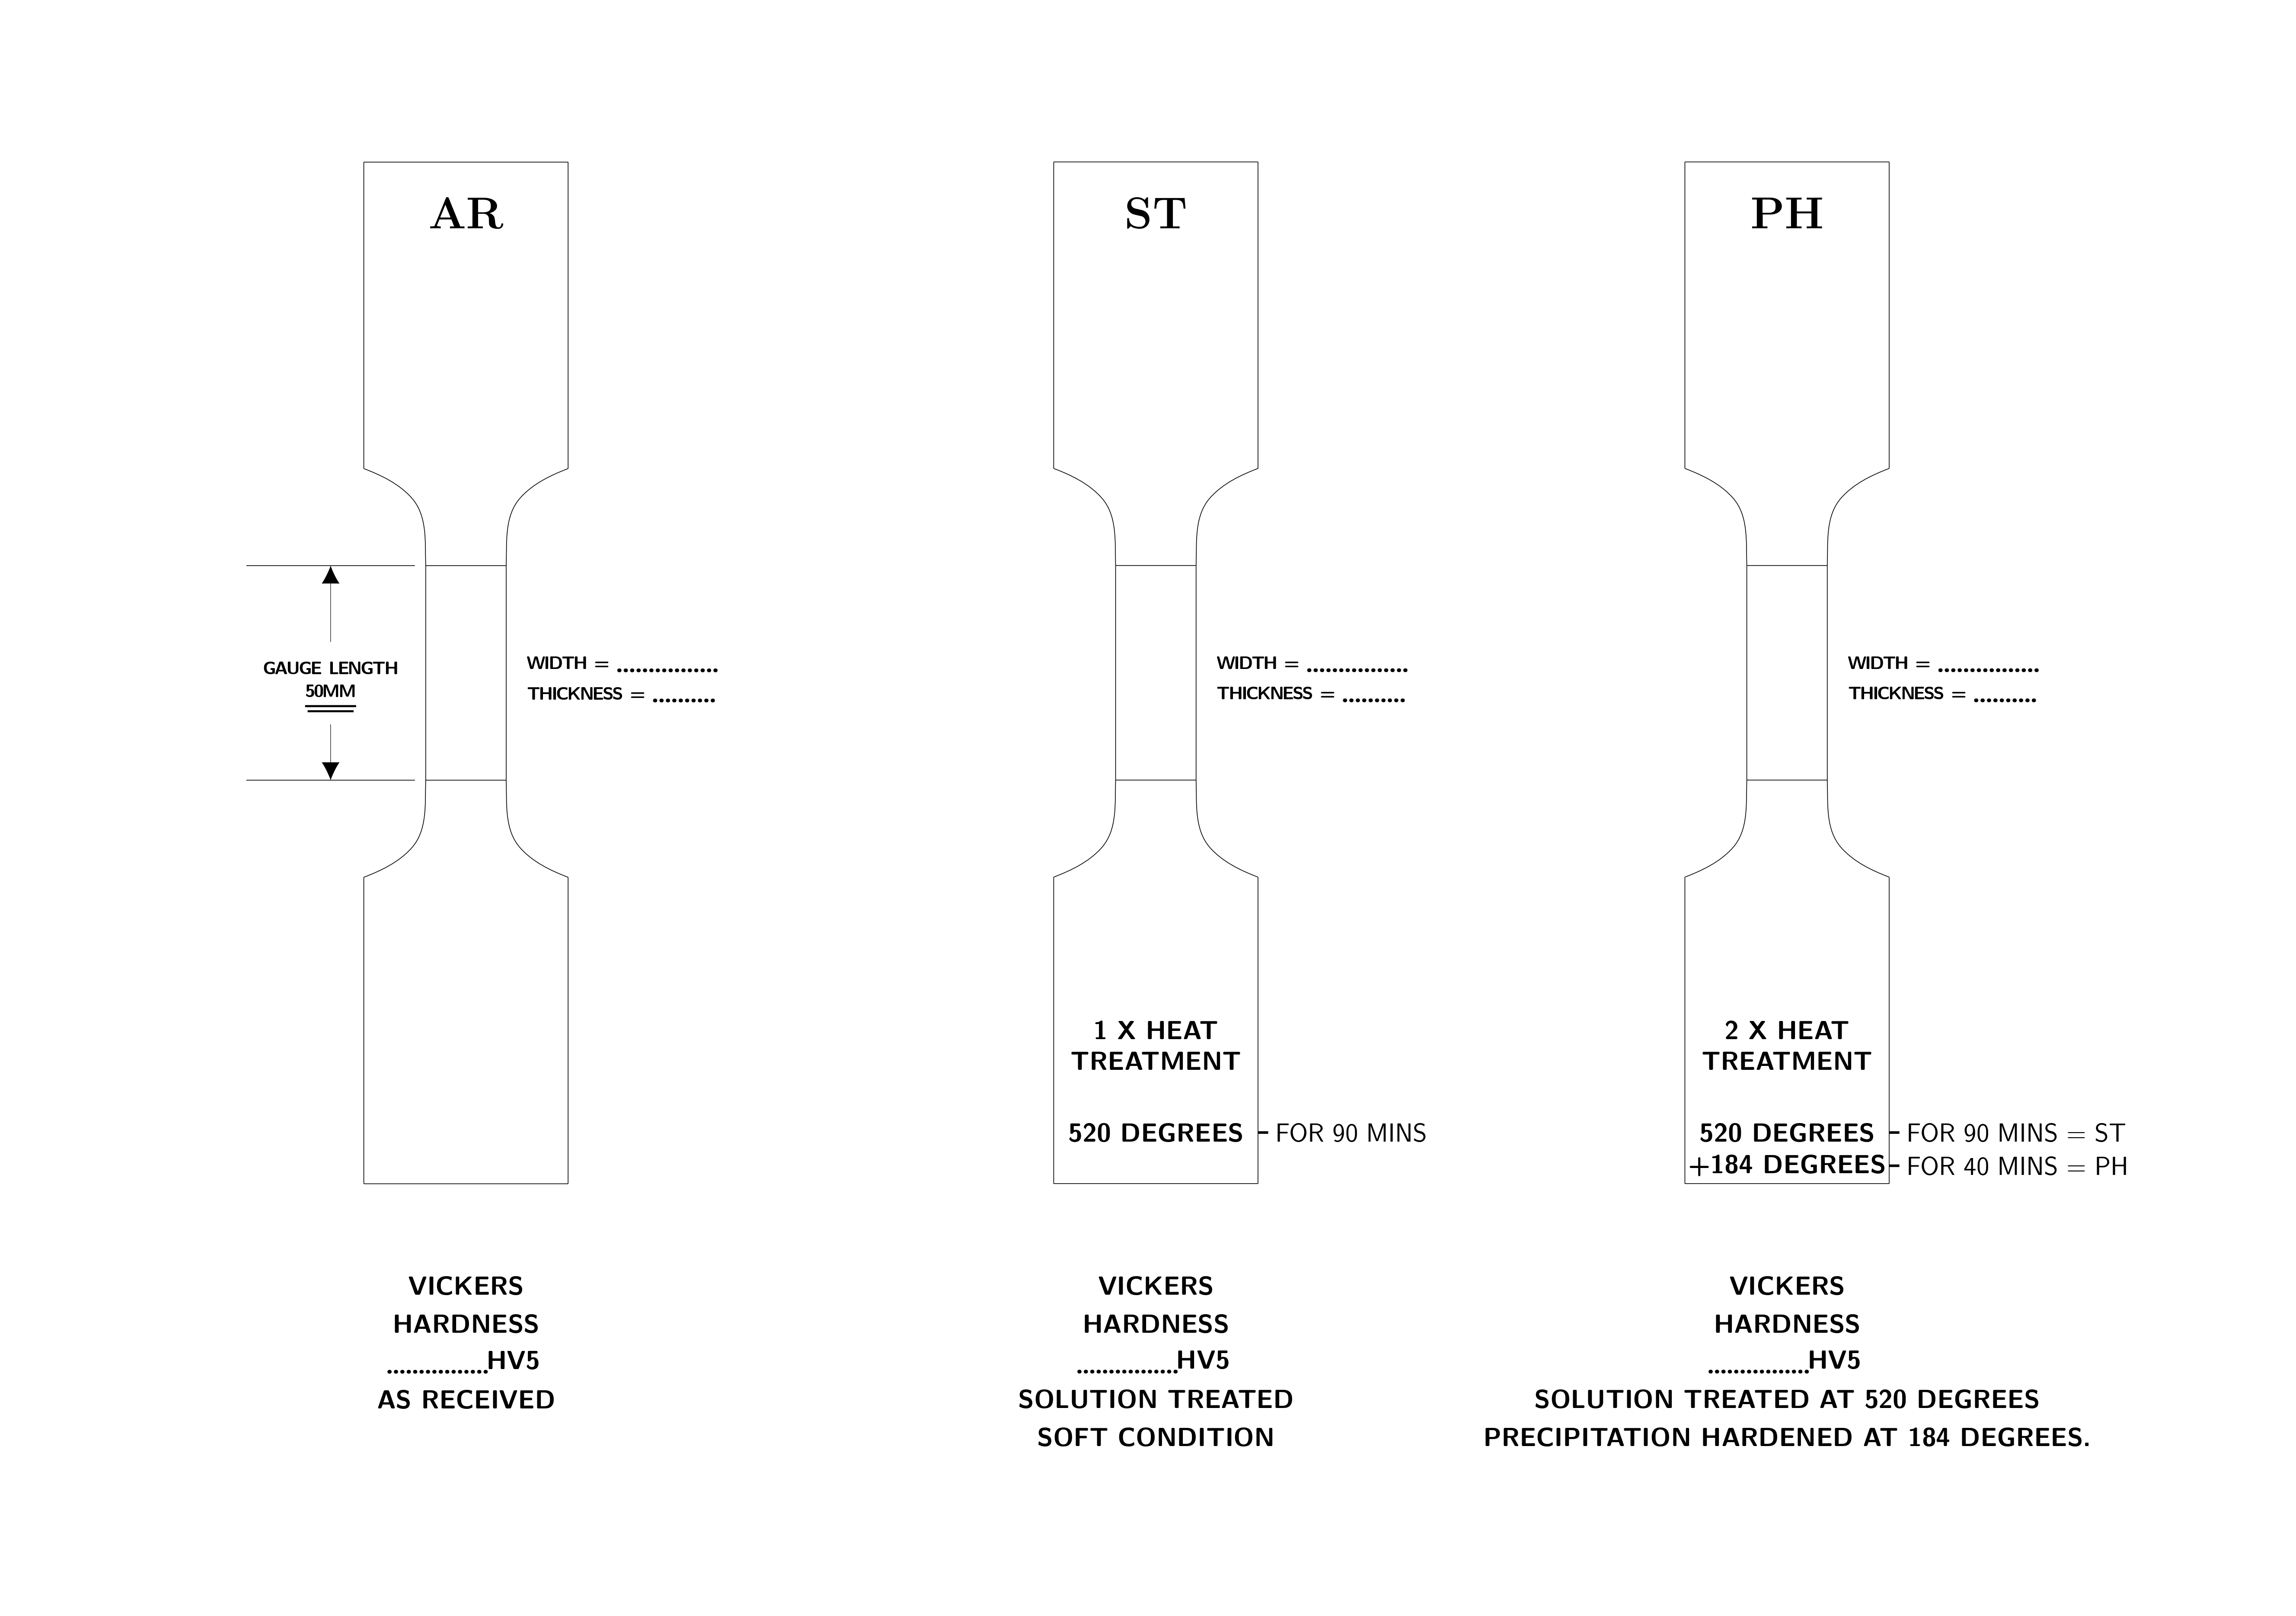
\includegraphics[width=0.98\textwidth,cfbox=gray!22 1pt]{figures/alloys_base.jpg} % LoL this shit would have been like 1k plus line at the least
    \caption{Form for recording sample measurements} 
    \label{fig:alloys} 
\end{figure}

\textbf{General Overview:}
The experiment was conducted in two phases: measuring the dimensions and hardness of alloy samples, followed by testing their tensile properties with the Zwick Roell 2050 Tensile Testing Machine. \\[8pt]
In the first phase, the width and length of each sample were recorded using digital calipers (in millimeters), while hardness was measured with a Vickers Hardness test machine using the HV5 scale. These tasks were conducted simultaneously, as both are quick and independent processes.\\[8pt]
After documenting the dimensions and hardness on the data sheet (See Figure \ref{fig:alloys}), we proceeded to the second phase of the experiment, were each sample was subjected to a controlled tensile force until fracture using the Zwick Roell 2050 Tensile Testing Machine. The data, including force applied and change in length, was recorded and summarized in a shared graph for all three alloys. This information was printed on an A4 sheet and given for additional examination outside of the lab (see Figure \ref{fig:tensile_results}). Important parameters, including yield strength, uts, stress, strain, and others, werecalculated after the experiment and are presented as a key part of analysis in this report.\\[8pt]
The following subsections detail the use of the equipment, outlining each step of the procedure and the results obtained at each stage.\\
\newpage
\begin{minipage}{0.32\textwidth}
\hspace{2em}
\begin{tikzpicture}[rotate around y=225, use Hobby shortcut,scale=0.35, every node/.style={scale=0.35}]
    \LARGE
    \def\width{4}
    \def\gap{10}
    \def\main{8}
    \def\curvy{1.9}
    \def\depth{3}
    
    \def\n{3.3}
    \def\z{1/\n}
    \pgfmathsetmacro{\s}{1-\z}
    
    \coordinate (A) at (0,\main,0);
    \coordinate (B) at (\width*\z-\width*\z*0.23,\main+\curvy-\curvy*0.7,0);
    \coordinate (C) at (\width*\z,\main+\curvy,0);
    
    \coordinate (A2) at (\width,\main,0);
    \coordinate (B2) at (\width*\s+\width*\z*0.23,\main+\curvy-\curvy*0.7,0);
    \coordinate (C2) at (\width*\s,\main+\curvy,0);
    
    \coordinate (A3) at (0,\main+\gap,0);
    \coordinate (B3) at (\width*\z-\width*\z*0.23,\main+\gap-\curvy+\curvy*0.7,0);
    \coordinate (C3) at (\width*\z,\main+\gap-\curvy,0);
    
    \coordinate (A4) at (\width,\main+\gap,0);
    \coordinate (B4) at (\width*\s+\width*\z*0.23,\main+\gap-\curvy+\curvy*0.7,0);
    \coordinate (C4) at (\width*\s,\main+\gap-\curvy,0);
    
    % Back variation with \depth (subtracting \depth from the z-coordinate)
    \coordinate (A') at (0,\main,\depth);
    \coordinate (B') at (\width*\z-\width*\z*0.23,\main+\curvy-\curvy*0.7,\depth);
    \coordinate (C') at (\width*\z,\main+\curvy,\depth);
    
    \coordinate (A2') at (\width,\main,\depth);
    \coordinate (B2') at (\width*\s+\width*\z*0.23,\main+\curvy-\curvy*0.7,\depth);
    \coordinate (C2') at (\width*\s,\main+\curvy,\depth);
    
    \coordinate (A3') at (0,\main+\gap,\depth);
    \coordinate (B3') at (\width*\z-\width*\z*0.23,\main+\gap-\curvy+\curvy*0.7,\depth);
    \coordinate (C3') at (\width*\z,\main+\gap-\curvy,\depth);
    
    \coordinate (A4') at (\width,\main+\gap,\depth);
    \coordinate (B4') at (\width*\s+\width*\z*0.23,\main+\gap-\curvy+\curvy*0.7,\depth);
    \coordinate (C4') at (\width*\s,\main+\gap-\curvy,\depth);
    
    
    % Back face fill
    \fill[black!40] 
    (0,0,\depth) -- (\width,0,\depth) -- (\width,\main,\depth) 
    to[hobby,tension=3] (\width,\main,\depth) .. (\width*\s+\width*\z*0.23,\main+\curvy-\curvy*0.7,\depth) .. (\width*\s,\main+\curvy,\depth) -- 
    (\width*\s,\main+\gap-\curvy,\depth) 
    to[hobby,tension=3] (\width*\s,\main+\gap-\curvy,\depth)  .. (\width*\s+\width*\z*0.23,\main+\gap-\curvy+\curvy*0.7,\depth) .. (\width,\main+\gap,\depth) --
    (\width,2*\main+\gap,\depth) -- (0,2*\main+\gap,\depth) -- 
    (0,\main+\gap,\depth) to[hobby,tension=3] (0,\main+\gap,\depth) .. (\width*\z-\width*\z*0.23,\main+\gap-\curvy+\curvy*0.7,\depth) .. (\width*\z,\main+\gap-\curvy,\depth) --
    (\width*\z,\main+\curvy,\depth) to[hobby,tension=3] (\width*\z,\main+\curvy,\depth) .. (\width*\z-\width*\z*0.23,\main+\curvy-\curvy*0.7,\depth) .. (0,\main,\depth) --
    cycle;
    
    % Curves fills with refined fades
    \fill[left color=gray!80, middle color=gray!50, right color=gray!20, opacity=0.8] 
    (A) to[hobby,tension=3] (A) .. (B) .. (C) -- (C3) to[hobby,tension=3] (C3) .. (B3) .. (A3) -- 
    (A3') to[hobby,tension=3] (A3') .. (B3') .. (C3') --
    (C') to[hobby,tension=3] (C') .. (B') .. (A') -- cycle;
    
    \fill[left color=gray!80, middle color=gray!50, right color=gray!20, opacity=0.8] 
    (A2) to[hobby,tension=3] (A2) .. (B2) .. (C2) -- (C4) to[hobby,tension=3] (C4) .. (B4) .. (A4) -- 
    (A4') to[hobby,tension=3] (A4') .. (B4') .. (C4') --
    (C2') to[hobby,tension=3] (C2') .. (B2') .. (A2') -- cycle;
    
    
    \draw[-,hobby,tension=3] (A2') .. (B2') .. (C2');
    \draw[-,hobby,tension=3] (A4') .. (B4') .. (C4');
    
    % Fill for bottom rectangle section
    \fill[black!33] 
    (0,0,0) -- (\width,0,0) -- (\width,0,\depth) -- (0,0,\depth) -- cycle;
    \fill[black!33] 
    (0,0,0) -- (0,\main,0) -- (0,\main,\depth) -- (0,0,\depth) -- cycle;
    \fill[black!40] 
    (\width,0,0) -- (\width,\main,0) -- (\width,\main,\depth) -- (\width,0,\depth) -- cycle;
    
    % Fill for top rectangle section
    \fill[black!30] 
    (0,2*\main+\gap,0) -- (\width,2*\main+\gap,0) -- (\width,2*\main+\gap,\depth) -- (0,2*\main+\gap,\depth) -- cycle;
    \fill[black!30] 
    (0,\main+\gap,0) -- (0,2*\main+\gap,0) -- (0,2*\main+\gap,\depth) -- (0,\main+\gap,\depth) -- cycle;
    \fill[black!33] 
    (\width,\main+\gap,0) -- (\width,2*\main+\gap,0) -- (\width,2*\main+\gap,\depth) -- (\width,\main+\gap,\depth) -- cycle;
    
    
    
    % Front face fill
    \fill[black!36] 
    (0,0,0) -- (\width,0,0) -- (\width,\main,0) 
    to[hobby,tension=3] (A2) .. (B2) .. (C2) -- 
    (\width*\s,\main+\gap-\curvy,0) 
    to[hobby,tension=3] (C4) .. (B4) .. (A4) --
    (\width,2*\main+\gap,0) -- (0,2*\main+\gap,0) -- 
    (0,\main+\gap,0) to[hobby,tension=3] (A3) .. (B3) .. (C3) --
    (\width*\z,\main+\curvy,0) to[hobby,tension=3] (C) .. (B) .. (A) --
    cycle;
    \draw[hobby,tension=3] (A) .. (B) .. (C);
    \draw[hobby,tension=3] (A2) .. (B2) .. (C2);
    \draw[hobby,tension=3] (A3) .. (B3) .. (C3);
    \draw[hobby,tension=3] (A4) .. (B4) .. (C4);
    \draw[dashed, opacity=0.3,hobby,tension=3] (A3') .. (B3') .. (C3');
    \draw[dashed, opacity=0.3,hobby,tension=3] (A') .. (B') .. (C');
    % Front face outline
    
    \draw[-] (0,0,0) -- (\width,0,0);
    \draw[-] (0,0,0) -- (0,\main,0);
    \draw[-] (\width*\z,\main+\curvy,0) -- (\width*\z,\main+\gap-\curvy,0);
    \draw[-] (0,\main+\gap,0) -- (0,2*\main+\gap,0);
    \draw[-] (0,2*\main+\gap,0) -- (\width,2*\main+\gap,0);
    \draw[-] (\width,2*\main+\gap,0) -- (\width,\main+\gap,0);
    \draw[-] (\width*\s,\main+\curvy,0) -- (\width*\s,\main+\gap-\curvy,0);    
    \draw[-] (\width,0,0) -- (\width,\main,0);
    
    
    
    
    
    % Back face outline
    
    
    \draw[dashed, opacity=0.3] (\width*\z,\main+\curvy,\depth) -- (\width*\z,\main+\gap-\curvy,\depth);
    \draw[-] (\width*\s,\main+\curvy,\depth) -- (\width*\s,\main+\gap-\curvy,\depth);
    \draw[dashed, opacity=0.3] (0,0,\depth) -- (\width,0,\depth);
    \draw[dashed, opacity=0.3] (0,0,\depth) -- (0,\main,\depth);
    \draw[-] (\width,0,\depth) -- (\width,\main,\depth);
    \draw[dashed, opacity=0.3] (0,\main+\gap,\depth) -- (0,2*\main+\gap,\depth);
    \draw[-] (0,2*\main+\gap,\depth) -- (\width,2*\main+\gap,\depth);
    \draw[-] (\width,2*\main+\gap,\depth) -- (\width,\main+\gap,\depth);
    
    
    
    % Connect front and back faces
    %botom
    \draw[-] (\width,\main,0) -- (\width,\main,\depth);
    \draw[-] (\width,0,0) -- (\width,0,\depth);
    \draw[dashed, opacity=0.3] (0,0,0) -- (0,0,\depth);
    \draw[-] (0,\main,0) -- (0,\main,\depth);
    %top
    \draw[-] (\width,\main+\gap,0) -- (\width,\main+\gap,\depth);
    \draw[-] (\width,2*\main+\gap,0) -- (\width,2*\main+\gap,\depth);
    \draw[-] (0,2*\main+\gap,0) -- (0,2*\main+\gap,\depth);
    \draw[dashed, opacity=0.3] (0,\main+\gap,0) -- (0,\main+\gap,\depth);
    
    
    
    %curves
    
    \draw[{Latex[length=1.93mm,width=1.93mm]}-{Latex[length=1.93mm,width=1.93mm]},line width=0.5mm] (C) -- (C2) node[below=-3,right=45] {\Huge \textbf{Width}};
    \draw[dashed, opacity=0.3] (C3) -- (C4);
    \draw[dashed, opacity=0.3] (C') -- (C2');
    \draw[dashed, opacity=0.3] (C3') -- (C4');
    \draw[dashed, opacity=0.3] (C) -- (C');
    \draw[{Latex[length=1.93mm,width=1.93mm]}-{Latex[length=1.93mm,width=1.93mm]},line width=0.5mm] (C2) -- (C2') node[below=-2,left] {\Huge \textbf{Thickness}};
    \draw[dashed, opacity=0.3] (C3) -- (C3');
    \draw[dashed, opacity=0.3] (C4) -- (C4');
    
    \draw[latex-latex, line width=0.5mm] 
    ($ (C) - (0.4,0,0) $) 
    -- ($ (C3) - (0.4,0,0) $) 
    node[right=5, midway] {\Huge \textbf{Length}};
    
\end{tikzpicture}
\end{minipage}\hfill
\begin{minipage}{0.65\textwidth}
\vspace{-1.5em}
\subsection{Measurements}\label{Measurements}
\vspace{0.5em}
\begin{center}
    \begin{tblr}{
        width=\textwidth,
        colspec={X[2,c]X[1,c]X[1,c]X[1,c]},
        hlines,vlines,
        rows={ht=1\baselineskip},
        row{1} = {ht=1\baselineskip,font=\bfseries,c,m},
        cells={valign=m,halign=c}
    }
    Property (mm) & AR & ST & PH \\
    Width   & 11.98 & 12.00 & 11.97 \\
    Thickness & 6.00  & 6.38  & 6.18  \\
    Length & 50.00 & 50.00 & 50.00 \\
\end{tblr}
\end{center}
\captionof{table}{Dimensions of AR, ST, and PH}
\label{tab:dimensions}
\vspace{1em}
\noindent
We measured the dimensions of each alloys gauge region using a digital calliper and recorded the results on the data sheet ( \ref{fig:alloys}). We were informed that the gauge length was 50 mm, but we did not measure it ourselves. Although checking measurements is good practice, this analysis does not require it because the gauge length has no bearing on the cross-sectional area (CSA), further explained below.
\end{minipage}\\
\vspace{1em}
\hspace{-2em}
\begin{minipage}{0.4\textwidth}
\hspace{2em}\begin{minipage}{0.3\textwidth} 
\centering
\begin{tikzpicture}[rotate around y=225, use Hobby shortcut, scale=0.25, every node/.style={scale=0.25}]
    \large
    \def\width{4}
    \def\gap{10}
    \def\main{8}
    \def\curvy{1.9}
    \def\depth{3}
    
    \def\n{3.3}
    \def\z{1/\n}
    \pgfmathsetmacro{\s}{1-\z}
    
    \coordinate (A) at (0,\main,0);
    \coordinate (B) at (\width*\z-\width*\z*0.23,\main+\curvy-\curvy*0.7,0);
    \coordinate (C) at (\width*\z,\main+\curvy,0);
    
    \coordinate (A2) at (\width,\main,0);
    \coordinate (B2) at (\width*\s+\width*\z*0.23,\main+\curvy-\curvy*0.7,0);
    \coordinate (C2) at (\width*\s,\main+\curvy,0);
    
    \coordinate (A3) at (0,\main+\gap,0);
    \coordinate (B3) at (\width*\z-\width*\z*0.23,\main+\gap-\curvy+\curvy*0.7,0);
    \coordinate (C3) at (\width*\z,\main+\gap-\curvy,0);
    
    \coordinate (A4) at (\width,\main+\gap,0);
    \coordinate (B4) at (\width*\s+\width*\z*0.23,\main+\gap-\curvy+\curvy*0.7,0);
    \coordinate (C4) at (\width*\s,\main+\gap-\curvy,0);
    
    % Back variation with \depth (subtracting \depth from the z-coordinate)
    \coordinate (A') at (0,\main,\depth);
    \coordinate (B') at (\width*\z-\width*\z*0.23,\main+\curvy-\curvy*0.7,\depth);
    \coordinate (C') at (\width*\z,\main+\curvy,\depth);
    
    \coordinate (A2') at (\width,\main,\depth);
    \coordinate (B2') at (\width*\s+\width*\z*0.23,\main+\curvy-\curvy*0.7,\depth);
    \coordinate (C2') at (\width*\s,\main+\curvy,\depth);
    
    \coordinate (A3') at (0,\main+\gap,\depth);
    \coordinate (B3') at (\width*\z-\width*\z*0.23,\main+\gap-\curvy+\curvy*0.7,\depth);
    \coordinate (C3') at (\width*\z,\main+\gap-\curvy,\depth);
    
    \coordinate (A4') at (\width,\main+\gap,\depth);
    \coordinate (B4') at (\width*\s+\width*\z*0.23,\main+\gap-\curvy+\curvy*0.7,\depth);
    \coordinate (C4') at (\width*\s,\main+\gap-\curvy,\depth);
    
    
    % Back face fill
    \fill[black!40] 
    (0,0,\depth) -- (\width,0,\depth) -- (\width,\main,\depth) 
    to[hobby,tension=3] (\width,\main,\depth) .. (\width*\s+\width*\z*0.23,\main+\curvy-\curvy*0.7,\depth) .. (\width*\s,\main+\curvy,\depth) -- 
    (\width*\s,\main+\gap-\curvy,\depth) 
    to[hobby,tension=3] (\width*\s,\main+\gap-\curvy,\depth)  .. (\width*\s+\width*\z*0.23,\main+\gap-\curvy+\curvy*0.7,\depth) .. (\width,\main+\gap,\depth) --
    (\width,2*\main+\gap,\depth) -- (0,2*\main+\gap,\depth) -- 
    (0,\main+\gap,\depth) to[hobby,tension=3] (0,\main+\gap,\depth) .. (\width*\z-\width*\z*0.23,\main+\gap-\curvy+\curvy*0.7,\depth) .. (\width*\z,\main+\gap-\curvy,\depth) --
    (\width*\z,\main+\curvy,\depth) to[hobby,tension=3] (\width*\z,\main+\curvy,\depth) .. (\width*\z-\width*\z*0.23,\main+\curvy-\curvy*0.7,\depth) .. (0,\main,\depth) --
    cycle;
    
    % Curves fills with refined fades
    \fill[left color=gray!80, middle color=gray!50, right color=gray!20, opacity=0.8] 
    (A) to[hobby,tension=3] (A) .. (B) .. (C) -- (C3) to[hobby,tension=3] (C3) .. (B3) .. (A3) -- 
    (A3') to[hobby,tension=3] (A3') .. (B3') .. (C3') --
    (C') to[hobby,tension=3] (C') .. (B') .. (A') -- cycle;
    
    \fill[left color=gray!80, middle color=gray!50, right color=gray!20, opacity=0.8] 
    (A2) to[hobby,tension=3] (A2) .. (B2) .. (C2) -- (C4) to[hobby,tension=3] (C4) .. (B4) .. (A4) -- 
    (A4') to[hobby,tension=3] (A4') .. (B4') .. (C4') --
    (C2') to[hobby,tension=3] (C2') .. (B2') .. (A2') -- cycle;
    
    
    \draw[-,hobby,tension=3] (A2') .. (B2') .. (C2');
    \draw[-,hobby,tension=3] (A4') .. (B4') .. (C4');
    
    % Fill for bottom rectangle section
    \fill[black!33] 
    (0,0,0) -- (\width,0,0) -- (\width,0,\depth) -- (0,0,\depth) -- cycle;
    \fill[black!33] 
    (0,0,0) -- (0,\main,0) -- (0,\main,\depth) -- (0,0,\depth) -- cycle;
    \fill[black!40] 
    (\width,0,0) -- (\width,\main,0) -- (\width,\main,\depth) -- (\width,0,\depth) -- cycle;
    
    % Fill for top rectangle section
    \fill[black!30] 
    (0,2*\main+\gap,0) -- (\width,2*\main+\gap,0) -- (\width,2*\main+\gap,\depth) -- (0,2*\main+\gap,\depth) -- cycle;
    \fill[black!30] 
    (0,\main+\gap,0) -- (0,2*\main+\gap,0) -- (0,2*\main+\gap,\depth) -- (0,\main+\gap,\depth) -- cycle;
    \fill[black!33] 
    (\width,\main+\gap,0) -- (\width,2*\main+\gap,0) -- (\width,2*\main+\gap,\depth) -- (\width,\main+\gap,\depth) -- cycle;
    
    
    
    % Front face fill
    \fill[black!36] 
    (0,0,0) -- (\width,0,0) -- (\width,\main,0) 
    to[hobby,tension=3] (A2) .. (B2) .. (C2) -- 
    (\width*\s,\main+\gap-\curvy,0) 
    to[hobby,tension=3] (C4) .. (B4) .. (A4) --
    (\width,2*\main+\gap,0) -- (0,2*\main+\gap,0) -- 
    (0,\main+\gap,0) to[hobby,tension=3] (A3) .. (B3) .. (C3) --
    (\width*\z,\main+\curvy,0) to[hobby,tension=3] (C) .. (B) .. (A) --
    cycle;
    \draw[hobby,tension=3] (A) .. (B) .. (C);
    \draw[hobby,tension=3] (A2) .. (B2) .. (C2);
    \draw[hobby,tension=3] (A3) .. (B3) .. (C3);
    \draw[hobby,tension=3] (A4) .. (B4) .. (C4);
    \draw[dashed, opacity=0.3,hobby,tension=3] (A3') .. (B3') .. (C3');
    \draw[dashed, opacity=0.3,hobby,tension=3] (A') .. (B') .. (C');
    % Front face outline
    
    \draw[-] (0,0,0) -- (\width,0,0);
    \draw[-] (0,0,0) -- (0,\main,0);
    \draw[-] (\width*\z,\main+\curvy,0) -- (\width*\z,\main+\gap-\curvy,0);
    \draw[-] (0,\main+\gap,0) -- (0,2*\main+\gap,0);
    \draw[-] (0,2*\main+\gap,0) -- (\width,2*\main+\gap,0);
    \draw[-] (\width,2*\main+\gap,0) -- (\width,\main+\gap,0);
    \draw[-] (\width*\s,\main+\curvy,0) -- (\width*\s,\main+\gap-\curvy,0);    
    \draw[-] (\width,0,0) -- (\width,\main,0);
    
    
    
    
    
    % Back face outline
    
    
    \draw[dashed, opacity=0.3] (\width*\z,\main+\curvy,\depth) -- (\width*\z,\main+\gap-\curvy,\depth);
    \draw[-] (\width*\s,\main+\curvy,\depth) -- (\width*\s,\main+\gap-\curvy,\depth);
    \draw[dashed, opacity=0.3] (0,0,\depth) -- (\width,0,\depth);
    \draw[dashed, opacity=0.3] (0,0,\depth) -- (0,\main,\depth);
    \draw[-] (\width,0,\depth) -- (\width,\main,\depth);
    \draw[dashed, opacity=0.3] (0,\main+\gap,\depth) -- (0,2*\main+\gap,\depth);
    \draw[-] (0,2*\main+\gap,\depth) -- (\width,2*\main+\gap,\depth);
    \draw[-] (\width,2*\main+\gap,\depth) -- (\width,\main+\gap,\depth);
    
    
    
    % Connect front and back faces
    %botom
    \draw[-] (\width,\main,0) -- (\width,\main,\depth);
    \draw[-] (\width,0,0) -- (\width,0,\depth);
    \draw[dashed, opacity=0.3] (0,0,0) -- (0,0,\depth);
    \draw[-] (0,\main,0) -- (0,\main,\depth);
    %top
    \draw[-] (\width,\main+\gap,0) -- (\width,\main+\gap,\depth);
    \draw[-] (\width,2*\main+\gap,0) -- (\width,2*\main+\gap,\depth);
    \draw[-] (0,2*\main+\gap,0) -- (0,2*\main+\gap,\depth);
    \draw[dashed, opacity=0.3] (0,\main+\gap,0) -- (0,\main+\gap,\depth);
    
    
    
    %curves
    \draw[dashed, opacity=0.3] (C) -- (C2);
    \draw[dashed, opacity=0.3] (C3) -- (C4);
    \draw[dashed, opacity=0.3] (C') -- (C2');
    \draw[dashed, opacity=0.3] (C3') -- (C4');
    \draw[dashed, opacity=0.3] (C) -- (C');
    \draw[dashed, opacity=0.3] (C2) -- (C2');
    \draw[dashed, opacity=0.3] (C3) -- (C3');
    \draw[dashed, opacity=0.3] (C4) -- (C4');
    
    
    \fill[opacity=0.6,pattern={Lines[
        distance=1mm,
        angle=45,
        line width=0.4mm
        ]},
    pattern color=blue
    ] (C2) -- (C) -- (C3) -- (C4) -- cycle;

\end{tikzpicture}
\color{blue} \textbf{\textsf{CSA 1}}
\end{minipage}\hspace{-1em}
\begin{minipage}{0.3\textwidth}
    \centering
    \begin{tikzpicture}[rotate around y=225, use Hobby shortcut, scale=0.25, every node/.style={scale=0.25}]
        \large
        \def\width{4}
        \def\gap{10}
        \def\main{8}
        \def\curvy{1.9}
        \def\depth{3}
        
        \def\n{3.3}
        \def\z{1/\n}
        \pgfmathsetmacro{\s}{1-\z}
        
        \coordinate (A) at (0,\main,0);
        \coordinate (B) at (\width*\z-\width*\z*0.23,\main+\curvy-\curvy*0.7,0);
        \coordinate (C) at (\width*\z,\main+\curvy,0);
        
        \coordinate (A2) at (\width,\main,0);
        \coordinate (B2) at (\width*\s+\width*\z*0.23,\main+\curvy-\curvy*0.7,0);
        \coordinate (C2) at (\width*\s,\main+\curvy,0);
        
        \coordinate (A3) at (0,\main+\gap,0);
        \coordinate (B3) at (\width*\z-\width*\z*0.23,\main+\gap-\curvy+\curvy*0.7,0);
        \coordinate (C3) at (\width*\z,\main+\gap-\curvy,0);
        
        \coordinate (A4) at (\width,\main+\gap,0);
        \coordinate (B4) at (\width*\s+\width*\z*0.23,\main+\gap-\curvy+\curvy*0.7,0);
        \coordinate (C4) at (\width*\s,\main+\gap-\curvy,0);
        
        % Back variation with \depth (subtracting \depth from the z-coordinate)
        \coordinate (A') at (0,\main,\depth);
        \coordinate (B') at (\width*\z-\width*\z*0.23,\main+\curvy-\curvy*0.7,\depth);
        \coordinate (C') at (\width*\z,\main+\curvy,\depth);
        
        \coordinate (A2') at (\width,\main,\depth);
        \coordinate (B2') at (\width*\s+\width*\z*0.23,\main+\curvy-\curvy*0.7,\depth);
        \coordinate (C2') at (\width*\s,\main+\curvy,\depth);
        
        \coordinate (A3') at (0,\main+\gap,\depth);
        \coordinate (B3') at (\width*\z-\width*\z*0.23,\main+\gap-\curvy+\curvy*0.7,\depth);
        \coordinate (C3') at (\width*\z,\main+\gap-\curvy,\depth);
        
        \coordinate (A4') at (\width,\main+\gap,\depth);
        \coordinate (B4') at (\width*\s+\width*\z*0.23,\main+\gap-\curvy+\curvy*0.7,\depth);
        \coordinate (C4') at (\width*\s,\main+\gap-\curvy,\depth);
        
        
        % Back face fill
        \fill[black!40] 
        (0,0,\depth) -- (\width,0,\depth) -- (\width,\main,\depth) 
        to[hobby,tension=3] (\width,\main,\depth) .. (\width*\s+\width*\z*0.23,\main+\curvy-\curvy*0.7,\depth) .. (\width*\s,\main+\curvy,\depth) -- 
        (\width*\s,\main+\gap-\curvy,\depth) 
        to[hobby,tension=3] (\width*\s,\main+\gap-\curvy,\depth)  .. (\width*\s+\width*\z*0.23,\main+\gap-\curvy+\curvy*0.7,\depth) .. (\width,\main+\gap,\depth) --
        (\width,2*\main+\gap,\depth) -- (0,2*\main+\gap,\depth) -- 
        (0,\main+\gap,\depth) to[hobby,tension=3] (0,\main+\gap,\depth) .. (\width*\z-\width*\z*0.23,\main+\gap-\curvy+\curvy*0.7,\depth) .. (\width*\z,\main+\gap-\curvy,\depth) --
        (\width*\z,\main+\curvy,\depth) to[hobby,tension=3] (\width*\z,\main+\curvy,\depth) .. (\width*\z-\width*\z*0.23,\main+\curvy-\curvy*0.7,\depth) .. (0,\main,\depth) --
        cycle;
        
        % Curves fills with refined fades
        \fill[left color=gray!80, middle color=gray!50, right color=gray!20, opacity=0.8] 
        (A) to[hobby,tension=3] (A) .. (B) .. (C) -- (C3) to[hobby,tension=3] (C3) .. (B3) .. (A3) -- 
        (A3') to[hobby,tension=3] (A3') .. (B3') .. (C3') --
        (C') to[hobby,tension=3] (C') .. (B') .. (A') -- cycle;
        
        \fill[left color=gray!80, middle color=gray!50, right color=gray!20, opacity=0.8] 
        (A2) to[hobby,tension=3] (A2) .. (B2) .. (C2) -- (C4) to[hobby,tension=3] (C4) .. (B4) .. (A4) -- 
        (A4') to[hobby,tension=3] (A4') .. (B4') .. (C4') --
        (C2') to[hobby,tension=3] (C2') .. (B2') .. (A2') -- cycle;
        
        
        \draw[-,hobby,tension=3] (A2') .. (B2') .. (C2');
        \draw[-,hobby,tension=3] (A4') .. (B4') .. (C4');
        
        % Fill for bottom rectangle section
        \fill[black!33] 
        (0,0,0) -- (\width,0,0) -- (\width,0,\depth) -- (0,0,\depth) -- cycle;
        \fill[black!33] 
        (0,0,0) -- (0,\main,0) -- (0,\main,\depth) -- (0,0,\depth) -- cycle;
        \fill[black!40] 
        (\width,0,0) -- (\width,\main,0) -- (\width,\main,\depth) -- (\width,0,\depth) -- cycle;
        
        % Fill for top rectangle section
        \fill[black!30] 
        (0,2*\main+\gap,0) -- (\width,2*\main+\gap,0) -- (\width,2*\main+\gap,\depth) -- (0,2*\main+\gap,\depth) -- cycle;
        \fill[black!30] 
        (0,\main+\gap,0) -- (0,2*\main+\gap,0) -- (0,2*\main+\gap,\depth) -- (0,\main+\gap,\depth) -- cycle;
        \fill[black!33] 
        (\width,\main+\gap,0) -- (\width,2*\main+\gap,0) -- (\width,2*\main+\gap,\depth) -- (\width,\main+\gap,\depth) -- cycle;
        
        
        
        % Front face fill
        \fill[black!36] 
        (0,0,0) -- (\width,0,0) -- (\width,\main,0) 
        to[hobby,tension=3] (A2) .. (B2) .. (C2) -- 
        (\width*\s,\main+\gap-\curvy,0) 
        to[hobby,tension=3] (C4) .. (B4) .. (A4) --
        (\width,2*\main+\gap,0) -- (0,2*\main+\gap,0) -- 
        (0,\main+\gap,0) to[hobby,tension=3] (A3) .. (B3) .. (C3) --
        (\width*\z,\main+\curvy,0) to[hobby,tension=3] (C) .. (B) .. (A) --
        cycle;
        \draw[hobby,tension=3] (A) .. (B) .. (C);
        \draw[hobby,tension=3] (A2) .. (B2) .. (C2);
        \draw[hobby,tension=3] (A3) .. (B3) .. (C3);
        \draw[hobby,tension=3] (A4) .. (B4) .. (C4);
        \draw[dashed, opacity=0.3,hobby,tension=3] (A3') .. (B3') .. (C3');
        \draw[dashed, opacity=0.3,hobby,tension=3] (A') .. (B') .. (C');
        % Front face outline
        
        \draw[-] (0,0,0) -- (\width,0,0);
        \draw[-] (0,0,0) -- (0,\main,0);
        \draw[-] (\width*\z,\main+\curvy,0) -- (\width*\z,\main+\gap-\curvy,0);
        \draw[-] (0,\main+\gap,0) -- (0,2*\main+\gap,0);
        \draw[-] (0,2*\main+\gap,0) -- (\width,2*\main+\gap,0);
        \draw[-] (\width,2*\main+\gap,0) -- (\width,\main+\gap,0);
        \draw[-] (\width*\s,\main+\curvy,0) -- (\width*\s,\main+\gap-\curvy,0);    
        \draw[-] (\width,0,0) -- (\width,\main,0);
        
        
        
        
        
        % Back face outline
        
        
        \draw[dashed, opacity=0.3] (\width*\z,\main+\curvy,\depth) -- (\width*\z,\main+\gap-\curvy,\depth);
        \draw[-] (\width*\s,\main+\curvy,\depth) -- (\width*\s,\main+\gap-\curvy,\depth);
        \draw[dashed, opacity=0.3] (0,0,\depth) -- (\width,0,\depth);
        \draw[dashed, opacity=0.3] (0,0,\depth) -- (0,\main,\depth);
        \draw[-] (\width,0,\depth) -- (\width,\main,\depth);
        \draw[dashed, opacity=0.3] (0,\main+\gap,\depth) -- (0,2*\main+\gap,\depth);
        \draw[-] (0,2*\main+\gap,\depth) -- (\width,2*\main+\gap,\depth);
        \draw[-] (\width,2*\main+\gap,\depth) -- (\width,\main+\gap,\depth);
        
        
        
        % Connect front and back faces
        %botom
        \draw[-] (\width,\main,0) -- (\width,\main,\depth);
        \draw[-] (\width,0,0) -- (\width,0,\depth);
        \draw[dashed, opacity=0.3] (0,0,0) -- (0,0,\depth);
        \draw[-] (0,\main,0) -- (0,\main,\depth);
        %top
        \draw[-] (\width,\main+\gap,0) -- (\width,\main+\gap,\depth);
        \draw[-] (\width,2*\main+\gap,0) -- (\width,2*\main+\gap,\depth);
        \draw[-] (0,2*\main+\gap,0) -- (0,2*\main+\gap,\depth);
        \draw[dashed, opacity=0.3] (0,\main+\gap,0) -- (0,\main+\gap,\depth);
        
        
        
        %curves
        \draw[dashed, opacity=0.3] (C) -- (C2);
        \draw[dashed, opacity=0.3] (C3) -- (C4);
        \draw[dashed, opacity=0.3] (C') -- (C2');
        \draw[dashed, opacity=0.3] (C3') -- (C4');
        \draw[dashed, opacity=0.3] (C) -- (C');
        \draw[dashed, opacity=0.3] (C2) -- (C2');
        \draw[dashed, opacity=0.3] (C3) -- (C3');
        \draw[dashed, opacity=0.3] (C4) -- (C4');
        
        
        \fill[opacity=0.6,pattern={Lines[
            distance=1mm,
            angle=45,
            line width=0.4mm
            ]},
        pattern color=green!70!black
        ] (C2) -- (C4) -- (C4') -- (C2') -- cycle;
    \end{tikzpicture}    
    \color{green!50!black} \textbf{\textsf{CSA 2}}
\end{minipage}\hspace{-1em}
\begin{minipage}{0.3\textwidth}
    \centering
    \begin{tikzpicture}[rotate around y=225, use Hobby shortcut, scale=0.25, every node/.style={scale=0.25}]
    \large
    \def\width{4}
    \def\gap{10}
    \def\main{8}
    \def\curvy{1.9}
    \def\depth{3}
    
    \def\n{3.3}
    \def\z{1/\n}
    \pgfmathsetmacro{\s}{1-\z}
    
    \coordinate (A) at (0,\main,0);
    \coordinate (B) at (\width*\z-\width*\z*0.23,\main+\curvy-\curvy*0.7,0);
    \coordinate (C) at (\width*\z,\main+\curvy,0);
    
    \coordinate (A2) at (\width,\main,0);
    \coordinate (B2) at (\width*\s+\width*\z*0.23,\main+\curvy-\curvy*0.7,0);
    \coordinate (C2) at (\width*\s,\main+\curvy,0);
    
    \coordinate (A3) at (0,\main+\gap,0);
    \coordinate (B3) at (\width*\z-\width*\z*0.23,\main+\gap-\curvy+\curvy*0.7,0);
    \coordinate (C3) at (\width*\z,\main+\gap-\curvy,0);
    
    \coordinate (A4) at (\width,\main+\gap,0);
    \coordinate (B4) at (\width*\s+\width*\z*0.23,\main+\gap-\curvy+\curvy*0.7,0);
    \coordinate (C4) at (\width*\s,\main+\gap-\curvy,0);
    
    % Back variation with \depth (subtracting \depth from the z-coordinate)
    \coordinate (A') at (0,\main,\depth);
    \coordinate (B') at (\width*\z-\width*\z*0.23,\main+\curvy-\curvy*0.7,\depth);
    \coordinate (C') at (\width*\z,\main+\curvy,\depth);
    
    \coordinate (A2') at (\width,\main,\depth);
    \coordinate (B2') at (\width*\s+\width*\z*0.23,\main+\curvy-\curvy*0.7,\depth);
    \coordinate (C2') at (\width*\s,\main+\curvy,\depth);
    
    \coordinate (A3') at (0,\main+\gap,\depth);
    \coordinate (B3') at (\width*\z-\width*\z*0.23,\main+\gap-\curvy+\curvy*0.7,\depth);
    \coordinate (C3') at (\width*\z,\main+\gap-\curvy,\depth);
    
    \coordinate (A4') at (\width,\main+\gap,\depth);
    \coordinate (B4') at (\width*\s+\width*\z*0.23,\main+\gap-\curvy+\curvy*0.7,\depth);
    \coordinate (C4') at (\width*\s,\main+\gap-\curvy,\depth);
    
    
    % Back face fill
    \fill[black!40] 
    (0,0,\depth) -- (\width,0,\depth) -- (\width,\main,\depth) 
    to[hobby,tension=3] (\width,\main,\depth) .. (\width*\s+\width*\z*0.23,\main+\curvy-\curvy*0.7,\depth) .. (\width*\s,\main+\curvy,\depth) -- 
    (\width*\s,\main+\gap-\curvy,\depth) 
    to[hobby,tension=3] (\width*\s,\main+\gap-\curvy,\depth)  .. (\width*\s+\width*\z*0.23,\main+\gap-\curvy+\curvy*0.7,\depth) .. (\width,\main+\gap,\depth) --
    (\width,2*\main+\gap,\depth) -- (0,2*\main+\gap,\depth) -- 
    (0,\main+\gap,\depth) to[hobby,tension=3] (0,\main+\gap,\depth) .. (\width*\z-\width*\z*0.23,\main+\gap-\curvy+\curvy*0.7,\depth) .. (\width*\z,\main+\gap-\curvy,\depth) --
    (\width*\z,\main+\curvy,\depth) to[hobby,tension=3] (\width*\z,\main+\curvy,\depth) .. (\width*\z-\width*\z*0.23,\main+\curvy-\curvy*0.7,\depth) .. (0,\main,\depth) --
    cycle;
    
    % Curves fills with refined fades
    \fill[left color=gray!80, middle color=gray!50, right color=gray!20, opacity=0.8] 
    (A) to[hobby,tension=3] (A) .. (B) .. (C) -- (C3) to[hobby,tension=3] (C3) .. (B3) .. (A3) -- 
    (A3') to[hobby,tension=3] (A3') .. (B3') .. (C3') --
    (C') to[hobby,tension=3] (C') .. (B') .. (A') -- cycle;
    
    \fill[left color=gray!80, middle color=gray!50, right color=gray!20, opacity=0.8] 
    (A2) to[hobby,tension=3] (A2) .. (B2) .. (C2) -- (C4) to[hobby,tension=3] (C4) .. (B4) .. (A4) -- 
    (A4') to[hobby,tension=3] (A4') .. (B4') .. (C4') --
    (C2') to[hobby,tension=3] (C2') .. (B2') .. (A2') -- cycle;
    
    
    \draw[-,hobby,tension=3] (A2') .. (B2') .. (C2');
    \draw[-,hobby,tension=3] (A4') .. (B4') .. (C4');
    
    % Fill for bottom rectangle section
    \fill[black!33] 
    (0,0,0) -- (\width,0,0) -- (\width,0,\depth) -- (0,0,\depth) -- cycle;
    \fill[black!33] 
    (0,0,0) -- (0,\main,0) -- (0,\main,\depth) -- (0,0,\depth) -- cycle;
    \fill[black!40] 
    (\width,0,0) -- (\width,\main,0) -- (\width,\main,\depth) -- (\width,0,\depth) -- cycle;
    
    % Fill for top rectangle section
    \fill[black!30] 
    (0,2*\main+\gap,0) -- (\width,2*\main+\gap,0) -- (\width,2*\main+\gap,\depth) -- (0,2*\main+\gap,\depth) -- cycle;
    \fill[black!30] 
    (0,\main+\gap,0) -- (0,2*\main+\gap,0) -- (0,2*\main+\gap,\depth) -- (0,\main+\gap,\depth) -- cycle;
    \fill[black!33] 
    (\width,\main+\gap,0) -- (\width,2*\main+\gap,0) -- (\width,2*\main+\gap,\depth) -- (\width,\main+\gap,\depth) -- cycle;
    
    
    
    % Front face fill
    \fill[black!36] 
    (0,0,0) -- (\width,0,0) -- (\width,\main,0) 
    to[hobby,tension=3] (A2) .. (B2) .. (C2) -- 
    (\width*\s,\main+\gap-\curvy,0) 
    to[hobby,tension=3] (C4) .. (B4) .. (A4) --
    (\width,2*\main+\gap,0) -- (0,2*\main+\gap,0) -- 
    (0,\main+\gap,0) to[hobby,tension=3] (A3) .. (B3) .. (C3) --
    (\width*\z,\main+\curvy,0) to[hobby,tension=3] (C) .. (B) .. (A) --
    cycle;
    \draw[hobby,tension=3] (A) .. (B) .. (C);
    \draw[hobby,tension=3] (A2) .. (B2) .. (C2);
    \draw[hobby,tension=3] (A3) .. (B3) .. (C3);
    \draw[hobby,tension=3] (A4) .. (B4) .. (C4);
    \draw[dashed, opacity=0.3,hobby,tension=3] (A3') .. (B3') .. (C3');
    \draw[dashed, opacity=0.3,hobby,tension=3] (A') .. (B') .. (C');
    % Front face outline
    
    \draw[-] (0,0,0) -- (\width,0,0);
    \draw[-] (0,0,0) -- (0,\main,0);
    \draw[-] (\width*\z,\main+\curvy,0) -- (\width*\z,\main+\gap-\curvy,0);
    \draw[-] (0,\main+\gap,0) -- (0,2*\main+\gap,0);
    \draw[-] (0,2*\main+\gap,0) -- (\width,2*\main+\gap,0);
    \draw[-] (\width,2*\main+\gap,0) -- (\width,\main+\gap,0);
    \draw[-] (\width*\s,\main+\curvy,0) -- (\width*\s,\main+\gap-\curvy,0);    
    \draw[-] (\width,0,0) -- (\width,\main,0);
    
    
    
    
    
    % Back face outline
    
    
    \draw[dashed, opacity=0.3] (\width*\z,\main+\curvy,\depth) -- (\width*\z,\main+\gap-\curvy,\depth);
    \draw[-] (\width*\s,\main+\curvy,\depth) -- (\width*\s,\main+\gap-\curvy,\depth);
    \draw[dashed, opacity=0.3] (0,0,\depth) -- (\width,0,\depth);
    \draw[dashed, opacity=0.3] (0,0,\depth) -- (0,\main,\depth);
    \draw[-] (\width,0,\depth) -- (\width,\main,\depth);
    \draw[dashed, opacity=0.3] (0,\main+\gap,\depth) -- (0,2*\main+\gap,\depth);
    \draw[-] (0,2*\main+\gap,\depth) -- (\width,2*\main+\gap,\depth);
    \draw[-] (\width,2*\main+\gap,\depth) -- (\width,\main+\gap,\depth);
    
    
    
    % Connect front and back faces
    %botom
    \draw[-] (\width,\main,0) -- (\width,\main,\depth);
    \draw[-] (\width,0,0) -- (\width,0,\depth);
    \draw[dashed, opacity=0.3] (0,0,0) -- (0,0,\depth);
    \draw[-] (0,\main,0) -- (0,\main,\depth);
    %top
    \draw[-] (\width,\main+\gap,0) -- (\width,\main+\gap,\depth);
    \draw[-] (\width,2*\main+\gap,0) -- (\width,2*\main+\gap,\depth);
    \draw[-] (0,2*\main+\gap,0) -- (0,2*\main+\gap,\depth);
    \draw[dashed, opacity=0.3] (0,\main+\gap,0) -- (0,\main+\gap,\depth);
    
    
    
    %curves
    \draw[dashed, opacity=0.3] (C) -- (C2);
    \draw[dashed, opacity=0.3] (C3) -- (C4);
    \draw[dashed, opacity=0.3] (C') -- (C2');
    \draw[dashed, opacity=0.3] (C3') -- (C4');
    \draw[dashed, opacity=0.3] (C) -- (C');
    \draw[dashed, opacity=0.3] (C2) -- (C2');
    \draw[dashed, opacity=0.3] (C3) -- (C3');
    \draw[dashed, opacity=0.3] (C4) -- (C4');
    
    \pgfmathsetmacro{\halfgap}{0.5*\gap}
    
    \coordinate (C3m) at (\width*\z,\main+\halfgap,0);
    \coordinate (C4m) at (\width*\s,\main+\halfgap,0);
    \coordinate (C3'm) at (\width*\z,\main+\halfgap,\depth);
    \coordinate (C4'm) at (\width*\s,\main+\halfgap,\depth);
    
    \fill[pattern={Lines[
        distance=1mm,
        angle=45,
        line width=0.4mm
        ]},
    pattern color=red,
    opacity=0.6] (C3m) -- (C3'm) -- (C4'm) -- (C4m) -- cycle;
\end{tikzpicture}
    \color{red} \textbf{\textsf{CSA 3}}
\end{minipage}
\end{minipage}
\begin{minipage}{0.63\textwidth}
    \vspace{-2em}
    \subsubsection{Cross-Sectional Areas (CSA)}
    \begin{center}
        \begin{tblr}{
                width=\textwidth,
                colspec={X[2.9,c]X[1.5,c]X[1.5,c]X[1.6,c]},
                hlines,vlines,
                rows={ht=1.5\baselineskip},
                row{1} = {ht=1\baselineskip,font=\bfseries,c,m},
                cells={valign=m,halign=c}
            }
            Property ($\bm{\text{mm}^2}$) & AR & ST & PH\\
            {\color{blue} \textbf{\textsf{CSA 1}} \\ Width \(\times\) Length} 
            & {\(11.98 \times 50\) \\ \(= 599\)} 
            & {\(12 \times 50\) \\ \(= 600\)} 
            & {\(11.97 \times 50\) \\ \(= 598.5\)} \\
            {\color{green!50!black} \textbf{\textsf{CSA 2}} \\ Thickness \(\times\) Length} 
            & {\(6 \times 50\) \\ \(= 300\)} 
            & {\(6.38 \times 50\) \\ \(= 319\)} 
            & {\(6.18 \times 50\) \\ \(= 309\)} \\
            {\color{red} \textbf{\textsf{CSA 3}} \\ Width \(\times\) Thickness} 
            & {\(11.98 \times 6\) \\ \(= 71.88\)} 
            & {\(12 \times 6.38\) \\ \(= 76.56\)} 
            & {\(11.97 \times 6.18\) \\ \(= 73.96\)} \\
        \end{tblr}
    \end{center}
    \captionof{table}{Calculated Cross-Sectional Areas (CSA) for AR, ST, and PH}
    \label{tab:csa}
    \vspace{1em}\noindent
    In a tensile test, force is applied from the top and bottom of the alloy, stretching it along its length. Stress is calculated as the force divided by the area \textbf{perpendicular} to the applied force. Thus, the appropriate cross-sectional area for stress calculation is the one that is perpendicular to this force.\footnotemark
\end{minipage}\\ \footnotetext{The calculations for the cross-sectional area (CSA) are conducted externally, not as part of the laboratory procedure, which is important for later context.}
\begin{itemize}[itemsep=-0.3mm]
    \item \textbf{\textcolor{blue}{\textsf{CSA 1}}:} This CSA parameterizes the thickness dimension of the alloy and remains coplanar with the applied force vector, rendering it unsuitable for stress calculations.
    \item \textbf{\textcolor{green!50!black}{\textsf{CSA 2}}:} This CSA parameterizes the width dimension and also remains coplanar with the applied force vector, thus it is not utilized for stress calculations.
    \item \textbf{\textcolor{red}{\textsf{CSA 3}}:} This CSA parameterizes the longitudinal dimension of the material and maintains orthogonality to the applied force vector, making it the appropriate choice for stress calculations.
\end{itemize}
\newpage
Thus, for stress calculations, we use \textbf{CSA 3}, as it is the area perpendicular to the applied force. The table below shows the calculated cross section area values for which is to be used.\vspace{1em}
\begin{center}
    \begin{tblr}{
            width=\textwidth,
            colspec={X[3,c]X[1.5,c]X[1.5,c]X[1.6,c]},
            hlines,vlines,
            rows={ht=1.3\baselineskip},
            row{1} = {ht=0.9\baselineskip,font=\bfseries,c,m},
            cells={valign=m,halign=c}
        }
        Property (\(\bm{\text{mm}^2}\)) & AR & ST & PH\\
        {\textbf{{Cross-Sectional Area}}} & 71.88 & 76.56& 73.96 \\
    \end{tblr}
\end{center}
\captionof{table}{Cross-Sectional Area (CSA) to be used for stress}
\label{tab:csa3}
\vspace{1em}\noindent
This data will be used in subsequent calculations for stress and other related analyses.
\subsection{Hardness Test}
To evaluate the hardness of our alloys, we employed the Vickers Hardness (HV) test, among others methods (See Section \ref{hardnesstypes}).\\[8pt]
The Vickers Hardness (HV) test is known as a precise and versatile method for measuring material hardness through indentation. It employs a diamond-shaped indenter with a square base at an included angle of 136\textdegree \ between opposing faces (See Figure \ref{fig:vickers-diagram}) (Ultramag, 2024; ZwickRoell, 2024).\\

\vspace{7pt}
\begin{minipage}{0.55\textwidth}
    The indenter is pressed into the material under a specific load, typically ranging from 1 to 100 kgf, applied for 10 to 15 seconds (Ultramag, 2024). In our case, we applied a load of 5N approximately 0.51 kgf for a duration of around 1-5 seconds presumably.\\[8pt]
    The process began by pressing the indenter onto the alloy surface, creating an indent. Afterward, using a dial, we adjusted the two parallel lines to align with the indent, measuring the first distance, \(d_1\), ensuring the indent was accurately positioned between the two sides (See Figure \ref{fig:vickers}). \\[8pt]  
    Once the first measurement was confirmed, we repositioned the sample and took the second distance measurement, \(d_2\), for the indent.\\[8pt]
    Finally, once both distances were recorded by the machine, we pressed a button to calculate the hardness.
\end{minipage}\hspace{1em}
\begin{minipage}{0.4\textwidth}\centering
\begin{figure}[H]
    \centering
    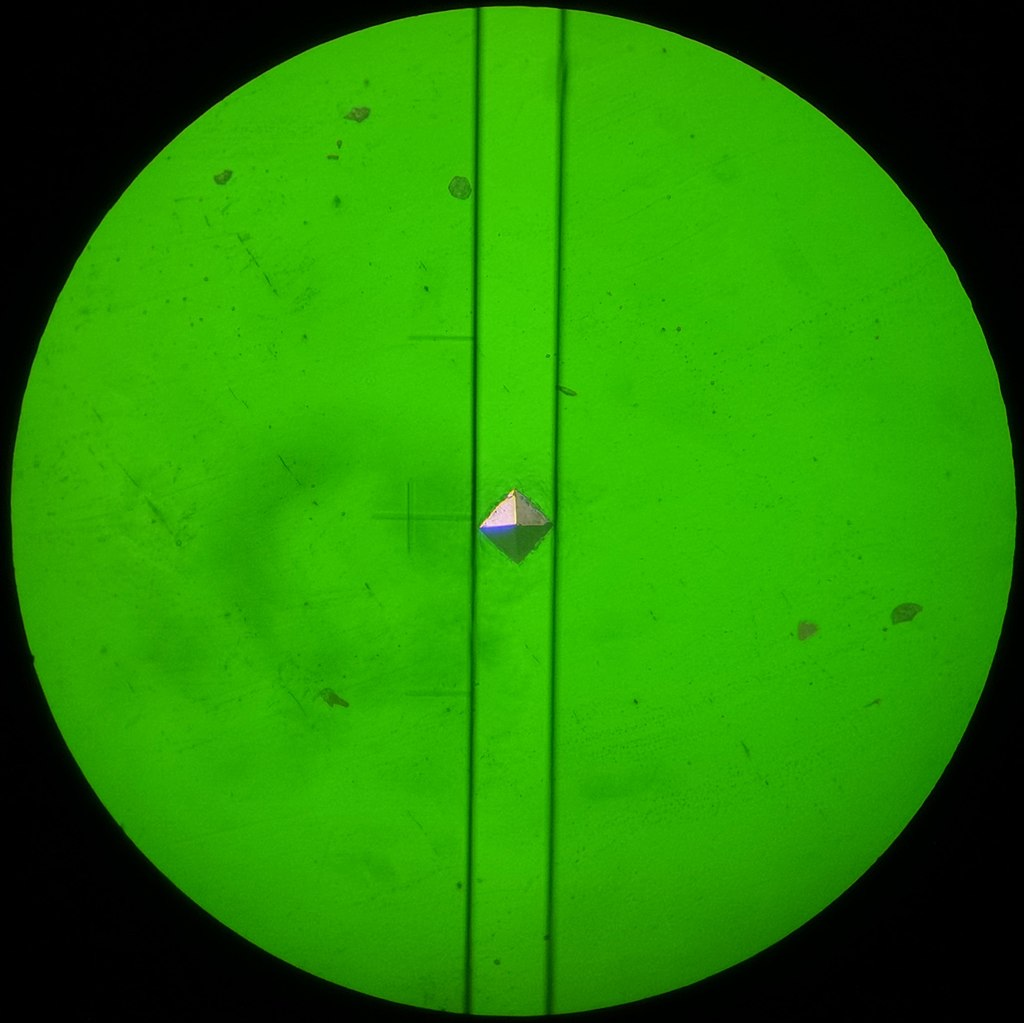
\includegraphics[width=0.8\textwidth]{images/1024px-Vicker_Hardness_-_Diamond_Indentation.jpg}
    \caption{Illustration showing the indent and the parallel lines used for measuring the indentation. (Wikipedia)}
    \label{fig:vickers}
\end{figure}
\end{minipage}\\
\vspace{10pt}
To ensure accuracy and consistency, this process was done at least 2-3 times for each given alloy and the resulting hardness values were recorded on the data sheet (See Figure \ref{fig:alloys}) for later analysis.\\[8pt]
Although the machine automatically calculates the hardness, it is important to understand the underlying process. The diagonals of the indentation $d_1$ and $d_2$ are used to calculate the Vickers hardness by determining the surface area of the indent. This area depends on the average of the two diagonal measurements, $d_1$ and $d_2$, as well as the geometry of the indentation. Together, these provide the necessary data to compute the material's hardness (ZwickRoell, 2024), i demonstrate and derive the pertinent equation and calculation for the HV5 test within theory section (See Section \ref{VHC}).
\newpage
The recorded results were documented on the data sheet (See Figure \ref{fig:alloys}) and were as follows:\\
\vspace{0.3em}
\begin{center}
    \begin{tblr}{
            width=\textwidth,
            colspec={X[3,c]X[0.75,c]X[0.75,c]X[0.75,c]X[0.75,c]X[0.75,c]X[0.75,c]X[0.8,c]X[0.8,c]X[0.8,c]},
            hlines,vlines,
            rows={ht=1\baselineskip},
            row{1} = {ht=1\baselineskip,font=\bfseries,c,m},
            cells={valign=m,halign=c}
        }
        Property (\(\bm{\text{unitless}}\)) & \SetCell[c=2]{c} AR & & \SetCell[c=2]{c} ST & & \SetCell[c=3]{c} PH & & \\
        HV5 (Individual) & 119 & 123 & 36 & 36.8 & 102.8 & 131 & 126 \\
    \end{tblr}
    \caption{HV5 Data}
    \label{tab:hv5}
\end{center}
\vspace{0.3em}
Table \ref{tab:hv5} shows the individual Vickers hardness (HV5) values for each alloy, with averages to be calculated using the mean formula (see Appendix C). A detailed analysis, including trends and implications, will follow in the Results section.\\[8pt]
\begin{minipage}{0.4\textwidth}
    \begin{figure}[H]
    \centering
    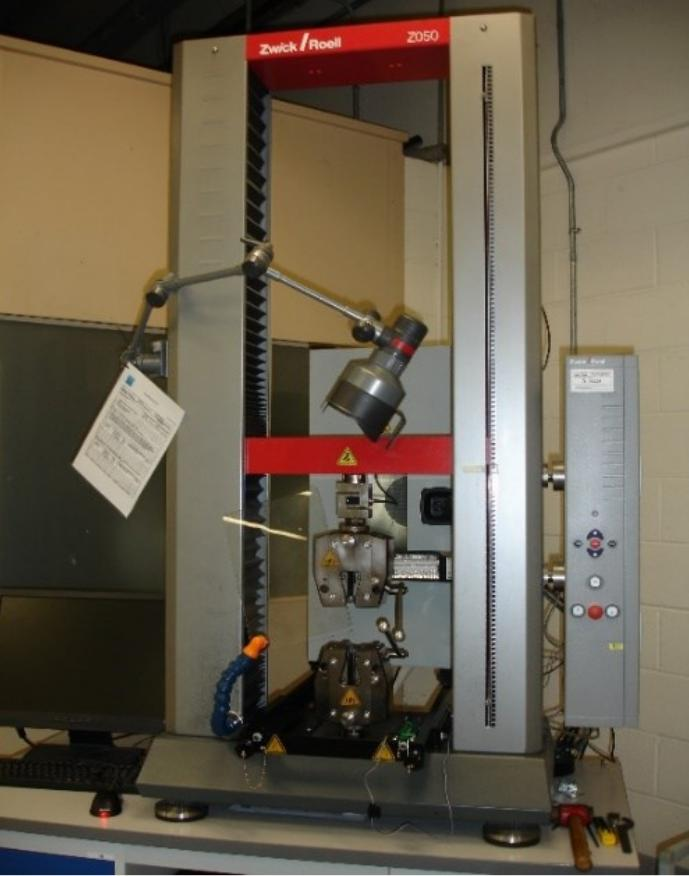
\includegraphics[width=0.8\textwidth]{images/tensile_machine.jpg}
    \caption{A Zwick tensile 50 kN testing similar to the used}
    \label{fig:tensile_machine}
    \end{figure}
\end{minipage}\hfill
\begin{minipage}{0.555\textwidth}
\subsection{Tensile Test}
This phase of the experiment focused tensile testing to assess the alloy's mechanical characteristics, particularly its tensile strength and elongation. The tensile tester used in this lab was a {Zwick machine}, with a maximum load capacity of 50 kN and an adjustable pulling rate (See Figure \ref{fig:tensile_machine}).\\[8pt]
An axial load was applied to the standardised dog-bone-shaped alloy as part of the destructive test procedure. The alloy, which had a precisely sized gauge length, was held firmly at both ends and extended at a regulated pace until it broke.\\[8pt]
For analysis, a real-time plot of force (N) versus change in length (mm) was generated during the experiment.
\end{minipage}\\[8pt]
Once the test was completed, i.e., after the specimen broke, the system also provided a table outlining details such as \textbf{Maximum Load (N)} \& \textbf{Extension at Break (mm)} \footnote{Table title terminology has been reworded for clarity. The original table titles are phrased strangely and incorrectly in a sense. A more detailed explanation and possible justification is provided in a later section.}. This process was automated using the manufacturer's software. The machine did not account for the sample's thickness or width, or simply by observation it was not given, making the data for these parameters invalid.\\[8pt]
Consequently, it is necessary for us to establish the relationship between the generated data and the initial measurements (e.g., cross-sectional area and original gauge length) (See Section \ref{Measurements}). While it may seem that providing the machine with the cross-sectional area and initial gauge length could have directly yielded a stress-strain curve, and correct data in the table, it is likely that this approach was deliberately avoided to encourage independent analysis and a deeper understanding of the process. There will be more discussion on this later on.

\newpage
\begin{figure}[H]
    \centering    
    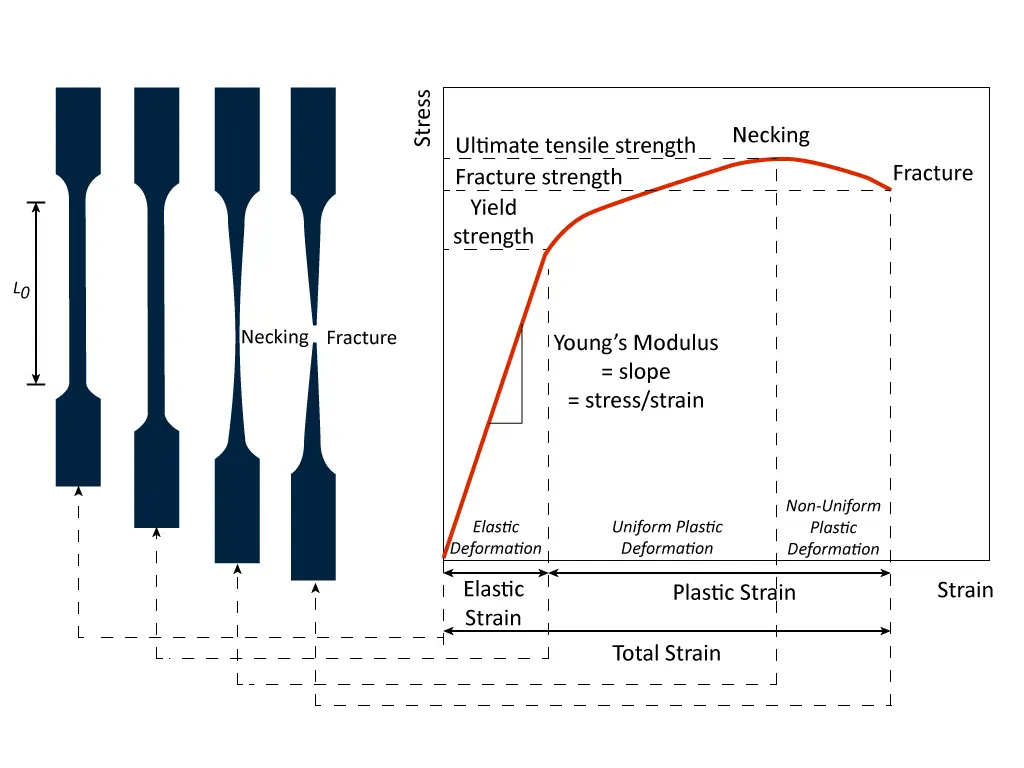
\includegraphics[width=0.7\textwidth]{images/simwiki-stress-strain-shape-evolution.png}
    \captionof{figure}{The shape of a ductile specimen changes during tensile testing (ADMET, 2017)}
    \label{fig:alloys_next_graph}
\end{figure}
This stress-strain graph, though not produced during our lab, illustrates key regions corresponding to visual changes in the alloy. While our real-time force vs. displacement graph isn't a true stress-strain curve, it represents similar principles due to proportional relationships. Thus, observed deformations can be linked to these stages. (For Further explanations see Section \ref{discuss}).\\[8pt]
The procedure followed during the tensile test was as follows: 
\begin{enumerate}
    \item We ensured all safety precautions, including wearing safety glasses and maintaining a safe distance (approximately 1.5 meters) from the equipment before starting the test.
    \item Upon initiating the test by clicking the "Start" button, the upper and lower grips moved in opposite directions according to the set pulling rate.
    \item The initial \textbf{elastic deformation region}, where the material experienced reversible stretching, was not noticeably perceptible in the alloys if not closely observant, due to the small change in length during this phase.\footnote{This region also corresponds to the Lüders region, where some materials undergo localized yielding before uniform plastic deformation. Whether this occurred in our alloy is uncertain, as I do not observe it in the graph produced by the machine (see Figure \ref{fig:tensile_results}). Regardless, no visible change in the material's shape or bands is seen during this phase.}
    \item Following the elastic region, the material enters the \textbf{uniform plastic deformation region}, where the material elongates uniformly across the specimen, and the elongation becomes more noticeable, with no localized necking occurring as of yet.
    \item The first noticeable event was \textbf{necking}, which visually manifests as a localized narrowing of the material at the gauge length region, indicating the onset of plastic deformation. This region is where the material started to stretch disproportionately at a certain point.
\end{enumerate}
\newpage
\begin{enumerate}
    \item[6.] Following necking, \textbf{non-uniform plastic deformation region}, the graph exhibited different behaviors (See Figure \ref{fig:stress_strain}) depending on the alloy being tested:
    \begin{itemize}
        \item For the solution-treated (ST) alloy, necking continued to propagate slowly, allowing further elongation before breaking, with the neck widening visibly before final failure.
        \item For the as-received (AR) and precipitation-hardened (PH) alloys, necking intensified rapidly, resulting in a more pronounced narrowing of the specimen and leading to quicker fracture.
    \end{itemize}
    The plot produced captured these differences, showing a sharp drop in force once the material reached its breaking point (See Figure \ref{fig:force_elong}).
\end{enumerate}
Once all three alloys broke, we were left with a shared force vs. displacement data and a table of results from the machine for all three alloys, this was to be printed all on an A4 sheet by ZwickRoell.\\ 
\vspace{3em}
\begin{center}
    \begin{minipage}{0.45\textwidth}
    \centering    
    \includegraphics[width=\textwidth]{images/image(6).jpeg}
    \captionof{figure}{The three broken alloys, showing the final stage of deformation after tensile testing.}
    \label{fig:broken_alloys}
\end{minipage}%
\hfil
\begin{minipage}{0.45\textwidth}
    \centering    
    \includegraphics[width=\textwidth]{example-image}
    \captionof{figure}{A4 machine data, including shared table and graph of alloys.}
    \label{fig:tensile_results}
     \footnotemark 
\end{minipage}
\end{center}
    \footnotetext{This is better represented in the Data and Result section}

   \newpage

    \section{Theory}
    
    In this section, I will outline the theoretical foundations underlying the methods and analyses used in this experiment. This includes the conceptual frameworks, mathematical models, and principles that explain the phenomena under investigation.\\[8pt]
    By detailing the reasoning behind the techniques and approaches employed, I aim to establish a solid foundation for the experimental procedures and data analysis, ensuring that the conclusions drawn are based on sound scientific principles.\\[8pt]
    Important theoretical ideas pertaining to our lab's work will be covered in this part, namely:
    \begin{itemize}
        \item \textbf{Hardness}
        \item \textbf{Tensile Testing}
        \begin{itemize}
            \item \textbf{Stress and Strain}
            \item \textbf{Young's Modulus} (also known as \textit{Modulus of Elasticity})
            \item \textbf{Ultimate Tensile Strength (UTS)}
            \item \textbf{Yield Strength and Elongation at Break}
            \item \textbf{Hooke's Law}
            \item \textbf{Poisson's Ratio}
            \item \textbf{Modulus of Resilience and Toughness}
            \item \textbf{Modulus of Toughness}
            \item \textbf{Slimness Ratio}
        \end{itemize}
    \end{itemize}
    Understanding all these properties will enable us to fully characterize the mechanical performance of the material under stress, allowing us to calculate them from the data collected during the experiment and fully assess our alloy.
    \newpage
       \subsection{Hardness}\label{hardnesstypes}
    Hardness is a material property that measures its resistance to deformation, scratching, or penetration by external forces. It is a critical factor in evaluating the durability and wear resistance of materials, often used in material science and engineering to determine suitability for specific applications.\\[8pt]
    The concept of hardness is multifaceted, encompassing several types:
    \begin{itemize}
        \item \textbf{Scratch Hardness}: The resistance of a material to scratching, often assessed using the Mohs scale, which ranks materials based on their ability to scratch one another.
        \item \textbf{Indentation Hardness}: This measures resistance to permanent deformation under localized pressure, typically using methods like the Brinell, Vickers, Rockwell or Knoop hardness tests.\footnote{Relevant equations and descriptions are shown at Appendix A}
        \item \textbf{Rebound Hardness}: The ability of a material to resist impact, evaluated through methods such as the Shore scleroscope test.
    \end{itemize}
    These approaches rely on different theoretical principles. For instance, indentation hardness tests use mathematical models to relate the force applied and the resulting deformation, often involving elastic and plastic deformation mechanics. The Mohs scale, on the other hand, is more qualitative and based on empirical observations.\\[8pt]
    Understanding hardness is essential in applications ranging from manufacturing to material selection, where wear resistance, strength, and surface durability are critical considerations.
    \subsubsection{Vickers Hardness Calculation}\label{VHC}
    \begin{figure}[H]
        \centering
        \begin{minipage}{0.45\textwidth}\centering
            \vspace{1em}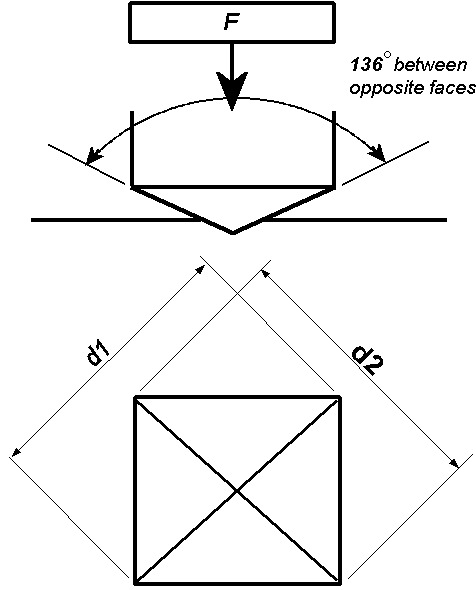
\includegraphics[width=0.8\textwidth]{figures/3537580_orig-0000.jpg}
            \caption{Diagram showing the diamond-shaped indenter with the 136° angle and diagonals \(d_1\) and \(d_2\).}
            \label{fig:vickers-diagram}
        \end{minipage}\hfill
        \begin{minipage}{0.51\textwidth}
            The Vickers hardness (HV) is calculated using the applied force (\(F\)) and the surface area (\(A\)) of the indentation. 
            \begin{equation}
                \text{HV} = \frac{F}{A}
            \end{equation}
            \begin{itemize}[itemsep=-1mm]
                \item HV: Vickers hardness (dimensionless)
                \item \(F\): Applied force (kgf or N)
                \item \(A\): Surface area of the indentation (mm\(^2\))
                
            \end{itemize}
            The formula for $A$ incorporates the geometry of the diamond pyramid indenter, 
            Such that surface area \(A\) can be expressed as:
            \begin{equation}
                A = \frac{d^2}{2\sin\left(\frac{136^\circ}{2}\right)} \approx \frac{d^2}{1.854} 
            \end{equation}
            Where:  
            \begin{itemize}[itemsep=-1mm]
                \item \(A\): Surface area of the indentation (mm\(^2\))
                \item \(d\): Arithmetic mean of the diagonals \(d_1\) and \(d_2\) (mm)
            \end{itemize}
            in so that it can be rewritten in terms of the diagonals as so:
            \begin{equation}
                A= \frac{\left(\frac{d_1+d_2}{2}\right)^2}{2\sin\left(\frac{136^\circ}{2}\right)} \approx \frac{\left(d_1 + d_2\right)^2}{7.236}
            \end{equation}
        \end{minipage}\\
    \end{figure}
    \vspace{-1em}\noindent
    Thus the derived formula is commonly shown as
    \begin{equation}
        {\text{HV} = \frac{F}{A} \approx \, \frac{1.854 \times F}{d^2} \approx \, \frac{7.236\times F}{\left(d_1 + d_2\right)^2}}    
    \end{equation} 
    The HV5 test we conducted applied a fixed load of 5 kgf (49.03 N), and the hardness was calculated via the machine as:  
    \begin{equation}
        \text{HV5} = \frac{49.03}{A} \approx \, \frac{90.902}{d^2} \approx \, \frac{354.781}{\left(d_1 + d_2\right)^2}
    \end{equation}
    Values for \(d_1\) and \(d_2\) were determined using the machine dial, and the corresponding hardness values were calculated based on them.\footnote{It is important to note that the resulting hardness value is expressed as a dimensionless number.}\\[8pt]
    \newpage

    \subsection{Tensile Testing}
    
    \begin{formal}[iqytechnicalcollege, 2012]
        Tensile testing is used to establish operational load limits for metals and alloys. A sample of the material is prepared so that a force can be applied along its axis. A central portion of the sample is reduced in width so that it will experience the highest stresses.\\[8pt]
        The tensile test measures the ability of a material to support a stress (force per unit area). The response of a tensile sample to the application of an increasing stress can be described in terms of elastic and plastic behavior. Initially, the sample undergoes elastic elongation as it is pulled. As increasing stress is applied, the sample undergoes permanent deformation; that is, plastic strain.\\[8pt]
        A stress-strain curve is used to determine the point at which the reversible elastic strain is exceeded and permanent or plastic deformation occurs. The yield strength is the stress necessary to cause significant plastic deformation (usually defined as 0.2\% strain).\\[8pt]
        Young’s modulus, or the modulus of elasticity, states the relationship between stress and strain represented by the straight-line portion of the stress-strain curve. It reflects the tendency of a material to deflect under a given applied stress.\\[8pt]
        Once yielding has begun, there is significant motion of dislocations within the metal grains. Grain boundaries, phase boundaries, and other dislocations hinder their movement. As more obstacles are encountered, the stress necessary to cause continued dislocation movement becomes greater. The maximum stress that the material can withstand before breaking is the ultimate tensile strength.\\[8pt]
        Reduction of area and percent elongation can be calculated from the broken sample. They are both indicators of a material’s ductility.\\
        \vspace{0.4pt}
    \end{formal}

     Stress and strain are fundamental concepts in tensile testing:\\[8pt]
     \subsection{Stress}
     \textbf{Stress} ($\sigma$) is the force divided by the cross-sectional area where that force is applied perpendicular to the material. In a tensile test, the area is constant (initial area $A_0$), while the applied force ($F$) changes, Mathematically, it is expressed as:\\[8pt]
            \begin{minipage}{0.48\textwidth}
            \begin{equation}
                \sigma = \frac{F}{A_9}
            \end{equation}
            where:
            \begin{itemize}[left=0pt,itemsep=-1mm]
                \item \( \sigma \): Stress, Pascals (Pa) or Newtons per meter squared (\(\text{N/m}^2\)),
                \item \( F \): Applied force, Newtons (N),
                \item \( A_0 \): Initial cross-sectional area, Meters squared (\(\text{m}^2\)).
            \end{itemize}
        \end{minipage}\hfill
        \begin{minipage}{0.48\textwidth}
            The original cross-sectional area is calculated as:
            \begin{equation}
                A_0 = w \times d
            \end{equation}
            where:
            \begin{itemize}[left=0pt,itemsep=-1mm]
                \item \( A_0 \): Initial cross-sectional area, Meters squared (\(\text{m}^2\)),
                \item \( w \): Width, Millimeters (mm),
                \item \( d \): Depth or thickness, Millimeters (mm).
            \end{itemize}
        \end{minipage}

        \subsection{Strain}
        \textbf{Strain} ($\varepsilon$) is a measure of the deformation of a material when it is subjected to stress. It is defined as the ratio of the change in length ($\Delta L$) to the original length ($L_0$) of the material. Unlike stress, strain is a dimensionless quantity, as it represents a relative change in length. Strain can be either elastic (reversible) or plastic (permanent), depending on the material's behavior during the application of the force, in terms of our tensile test the lengths here our related to alloys gauge, Mathematically, it is expressed as:\\[8pt]        
        \begin{minipage}{0.48\textwidth}
            \begin{equation}
                \varepsilon = \frac{\Delta L}{L_0}
            \end{equation}
            Where:
            \begin{itemize}[left=0pt,itemsep=-1mm]
                \item \( \varepsilon \): Strain, a dimensionless quantity (no units).
                \item \( \Delta L \): Change in length, meters (m).
                \item \( L_0 \): Original length, meters (m).
            \end{itemize}
        \end{minipage}\hfill
        \begin{minipage}{0.48\textwidth}
            The change in length (\( \Delta L \)) is calculated as:
            \begin{equation}
                \Delta L = \left| L - L_0 \right|
            \end{equation}
            where:
            \begin{itemize}[left=0pt,itemsep=-1mm]
                \item \( \Delta L \): Change in length, meters (m),
                \item \( L \): Current length, meters (m),
                \item \( L_0 \): Original length, meters (m).
            \end{itemize}
        \end{minipage}
        

        
    \subsection{Young's Modulus}
    \textbf{Young's Modulus} (\(E\)) also known as \textit{Modulus of Elasticity} is a material constant that quantifies the stiffness of a material in the elastic region. Mathematically, it is expressed as:\\[8pt]
    \begin{equation}
        E = \frac{\sigma}{\varepsilon}
    \end{equation}
    Where:
    \begin{itemize}
        \item \( E \): Young's modulus, Pascals (Pa) or Newtons per meter squared (\(\text{N/m}^2\)).
        \item \( \sigma \): Stress Pascals (Pa) or Newtons per meter squared (\(\text{N/m}^2\)).
        \item \( \varepsilon \): Strain, a dimensionless quantity (no units).
    \end{itemize}
        
    \subsection{Ultimate Tensile Strength (UTS)}
    % Add content here
    
    \subsection{Yield Strength and Elongation at Break}
    % Add content here
    
    \subsection{Hooke's Law}
    % Add content here
    
    \subsection{Poisson's Ratio}
    % Add content here
    
    \subsection{Modulus of Resilience and Toughness}
    % Add content here
    
    \subsection{Modulus of Toughness}
    % Add content here
    
    \subsection{Slimness Ratio}
    % Add content here




    
    
    \newpage\vspace*{-20pt}
    
    \section{Data and Result Calculations}
    
    Now that we have the following data:
    \begin{itemize}
        \item Gauge dimensions
        \item Hardness (v5)
        \item Force vs. elongation graph
    \end{itemize}
    We can now derive several mechanical properties:
    
    These derived properties will help us fully characterize the mechanical performance of the material under stress.
    \newpage
    \subsection{hardness data}
    \begin{center}
        \begin{tblr}{
                width=\textwidth,
                colspec={X[3,c]X[0.75,c]X[0.75,c]X[0.75,c]X[0.75,c]X[0.75,c]X[0.75,c]X[0.8,c]X[0.8,c]X[0.8,c]},
                hlines,vlines,
                rows={ht=1\baselineskip},
                row{1} = {ht=1\baselineskip,font=\bfseries,c,m},
                cells={valign=m,halign=c}
            }
            Property (\(\bm{\text{unitless}}\)) & \SetCell[c=2]{c} AR & & \SetCell[c=2]{c} ST & & \SetCell[c=3]{c} PH & & \\
            HV5 (Individual) & 119 & 123 & 36 & 36.8 & 102.8 & 131 & 126 \\
        \end{tblr}
    \end{center}
    To calculate the mean (or average) for each set of values, 
    sum all individual values and divide by the total number of values, as shown by the formula:
    \begin{equation}
        \text{Mean} = \frac{\sum x_i}{n}
    \end{equation}
    Where:
    \begin{itemize}[itemsep=-1mm]
        \item \textbf{Mean}: The arithmetic average, representing the central tendency of the dataset.
        \item \( x_i \): Each individual value in the dataset.
        \item \( n \): The total number of values in the dataset.
        \item \( \sum x_i \): The sum of all individual values.
    \end{itemize}
    Before calculating the mean, it is important to identify and remove outliers. 
    During the lab, it was determined that the value 102.8 from PH was an outlier. 
    With this adjustment, the results can now proceed as follows:\\
    \begin{center}
        \textbf{AR:}
        \[\sum x_i = 119 + 123 = 242\]
        \[n = 2 \quad \Rightarrow \quad \text{Mean} = \frac{242}{2} = 121\]
        \textbf{ST:}
        \[\sum x_i = 36 + 36.8 = 72.8\]
        \[n = 2 \quad \Rightarrow \quad \text{Mean} = \frac{72.8}{2} = 36.4\]
        \textbf{PH:}
        \[\sum x_i = 131 + 126 = 257\]
        \[n = 2 \quad \Rightarrow \quad \text{Mean} = \frac{257}{2} = 128.5\]
    \end{center}    
Thus, the means for each group are as follows:
    \begin{center}
        \begin{tblr}{
                width=\textwidth,
                colspec={X[3,c]X[0.75,c]X[0.75,c]X[0.75,c]X[0.75,c]X[0.75,c]X[0.75,c]X[0.8,c]X[0.8,c]X[0.8,c]},
                hlines,vlines,
                rows={ht=1\baselineskip},
                row{1} = {ht=1\baselineskip,font=\bfseries,c,m},
                cells={valign=m,halign=c}
            }
            Property (\(\bm{\text{unitless}}\)) & \SetCell[c=2]{c} AR & & \SetCell[c=2]{c} ST & & \SetCell[c=3]{c} PH & & \\
            HV5 (Individual) & 119 & 123 & 36 & 36.8 & \(\cancel{102.8}\) & 131 & 126 \\
            HV5 (Average) & \SetCell[c=2]{c} 121 & & \SetCell[c=2]{c} 36.4 & & \SetCell[c=3]{c} 128.5 & & \\
        \end{tblr}
        \caption{HV5 individual and mean data}
        \label{tab:hv5mean}
    \end{center}
    \subsection{Force vs Displacement}
    
        \renewcommand{\arraystretch}{1.4}
        \begin{table}[H]
            \centering
            \begin{tblr}{
                    width=\textwidth,
                    colspec={X[0.4,c]X[1,c]X[1.1,c]X[1.9,c]X[1.9,c]X[1.1,c]X[0.8,c]X[0.7,c]},
                    hlines,vlines,
                    cells={valign=m,halign=c}
                }
                \textbf{Nr} & \textbf{Specimen ID} & \textbf{Date} & \textbf{Stress - Maximum Load (N)} & \textbf{Strain Extension at Break (mm)} & \textbf{Thickness (mm)} & \textbf{Width (mm)} & \textbf{CSA \((\text{mm}^2)\)} \\
                1 & ST & 20/11/2024 & 8580 & 19.8 & 1 & 1 & 1.00 \\
                2 & PH & 20/11/2024 & 23800 & 9.8 & 1 & 1 & 1.00 \\
                3 & AR & 20/11/2024 & 24400 & 9.7 & 1 & 1 & 1.00 \\
                \end{tblr}
            \caption{Specimen Data}
            \label{tab:specimen_data}
        \end{table}

    \begin{figure}[H]
        \centering
\includegraphics[width=0.7\textwidth]{figures/force_vs_elongation.png}       
\caption{Machine produced data for Force vs Elongation}
        \label{fig:force_elong}
    \end{figure}
    \subsection{Stress vs Strain}
    \begin{figure}[H]
    \centering
    \includegraphics[width=0.7\textwidth]{figures/stress_vs_strain.png}
    \caption{Calculated produced data for Stress vs Strain}
    \label{fig:stress_strain}
\end{figure}    

        
    \newpage\vspace*{-5pt}
    \section{Discussion}\label{discuss}
    The similarity between the Force vs Elongation graph and the Stress vs Strain graph arises from the underlying relationship between force, elongation, stress, and strain. In the Force vs Elongation graph, force (in Newtons) is plotted against the change in length (elongation, in millimeters), showing the direct relationship between the applied load and the resulting deformation. However, in the Stress vs Strain graph, both force and elongation are scaled down by constants: force is divided by the cross-sectional area of the specimen, and elongation is divided by the original gauge length of the specimen. This scaling reduces the magnitude of the values in the Stress vs Strain graph, which is why the graph appears smaller, even though the overall shape and behavior are similar. Specifically, stress represents force per unit area, and strain represents the relative change in length, both of which are dimensionless or have smaller units compared to force and elongation. Therefore, the difference in graph scales is simply due to this division by constants, which doesn't affect the overall shape of the curve but rather scales the values down, making the Stress vs Strain graph appear "smaller" than the Force vs Elongation graph.
    \newpage\vspace*{-5pt}
    \section{Conclusions}

    \newpage\vspace*{-5pt}
    \section{Recommendations}

    \newpage\vspace*{-5pt}
    \section{References}
    \begin{enumerate}
        \item Eurotherm (2024) \textit{An Introduction to the Heat Treatment of Metallic Alloys}. Available at: \url{https://www.eurotherm.com/sv/heat-treatment-articles-sv/an-introduction-to-the-heat-treatment-of-metallic-alloys/} [Accessed 19 December 2024].
        
        \item Rajaa, S. M., Abdulhadi, H. A., Jabur, K. S., and Mohammed, G. R. (2018). Aging Time Effects on the Mechanical Properties of Al 6061-T6 Alloy. Available at: \url{https://pdfs.semanticscholar.org/a99b/8b7e771be0fecaaeb970074c7a2871a77032.pdf} [Accessed 19 December 2024].        

        \item Singh, P., Singh, R.K. \& Das, A.K. (2023) \textit{‘Optimization of Heat Treatment Cycle for Cast-Al6082 Alloy to Enhance the Mechanical Properties’}. Research Square. Available at: \url{https://assets-eu.researchsquare.com/files/rs-3363991/v1/9cd60f8c-a164-4e04-8552-1933478eaded.pdf?c=1711467707} [Accessed 7 December 2024].
        
        \item Thyssenkrupp Materials (2023) \textit{Aerospace Grade Aluminium}. Available at: \url{https://www.thyssenkrupp-materials.co.uk/aerospace-grade-aluminum} [Accessed 19 December 2024].
        
        \item Truventor (2019) \textit{Aluminium 6082 Data Sheet}. Available at: \url{https://truventor.ai/assets/pdf/datasheets/Aluminium%206082.pdf} [Accessed 19 December 2024].
        
        \item Rovida, C., Alépée, N., Api, A.M., Basketter, D.A., Bois, F.Y., Caloni, F., Corsini, E., Daneshian, M., Eskes, C., Ezendam, J., Fuchs, H., Hayden, P., Hegele-Hartung, C., Hoffmann, S., Hubesch, B., Jacobs, M.N., Jaworska, J., Kleensang, A., Kleinstreuer, N., Lalko, J., Landsiedel, R., Lebreux, F., Luechtefeld, T., Locatelli, M., Mehling, A., Natsch, A., Pitchford, J.W., Prater, D., Prieto, P., Schepky, A., Schüürmann, G., Smirnova, L., Toole, C., van Vliet, E., Weisensee, D. and Hartung, T. (2015) \textit{Integrated Testing Strategies (ITS) for Safety Assessment}. Available at: \url{https://www.researchgate.net/publication/6538912_The_Principles_of_Weight_of_Evidence_Validation_of_Test_Methods_and_Testing_Strategies_The_Report_and_Recommendations_of_ECVAM_Workshop_58} [Accessed 20 December 2024].
        
        \item Alan Turing Institute (2024) \textit{Data-Driven Experiment Design}. Available at: \url{https://www.turing.ac.uk/research/research-projects/data-driven-experiment-design} [Accessed 20 December 2024].
        
        
       % alloy image
        % https://www.admet.com/blog/effect-specimen-geometry-tensile-testing-results/
        
       % vickesrs hardness
        %https://www.ultramag.co.uk/ndt-inspection/hardness-testing/
        %https://www.zwickroell.com/industries/metals/metals-standards/vickers-test-iso-6507/
        
        % confirmation clari
        % https://www.actonbrightsteel.co.uk/6082-t6-acton-bright-steel.html
        
        % compisition
        % file:///home/sak/Downloads/Aalco-Metals-Ltd_Aluminium-Alloy-6082-T6T651-Plate_148.pdf
        % https://www.aalco.co.uk/datasheets/Aluminium-Alloy_6082-T6~T651_148.ashx
    \end{enumerate}

    
    
    %https://nasruldesign.weebly.com/ndt---brief-overview.html
    %https://www.sciencedirect.com/topics/materials-science/indentation-hardness-testing
    %https://nasruldesign.weebly.com/uploads/7/4/1/9/7419180/hardness_testing_manual.pdf
    

    \newpage\vspace*{-5pt}
    
   
    
\section{Appendix}
\normalsize
\renewcommand{\thesubsection}{\Alph{subsection}}

\subsection{Indentation hardness types}
The Brinell Hardness Number (BHN) measures a material's resistance to deformation, determined by the indentation left by a hard steel or carbide ball pressed into the material under a specified load. This test is commonly used for materials with a coarse or heterogeneous grain structure.\\[1em]
The formula for calculating the Brinell Hardness Number is:
\begin{equation}
    BHN = \frac{2P}{\pi D (D - \sqrt{D^2 - d^2})}
\end{equation}
Where:
\begin{itemize}[itemsep=-1mm]
    \item \( P \) : applied load in kilogram-force (kgf),
    \item \( D \) : diameter of the indenter (typically 10 mm),
    \item \( d \) : diameter of the indentation (mm).
\end{itemize}
\textbf{Note}: The Brinell test may use either $P$ or $F$ for the load, depending on the source.\\ 
The BHN provides insight into a material's ability to resist wear and deformation, which is important for assessing the durability and suitability of metals in various engineering applications. BHN values are particularly useful for testing larger, rougher materials and are commonly applied to metals like steel and cast iron. The results help predict wear resistance and strength under load.


\subsection{RSM and FFS}
\textbf{Response Surface Methodology (RSM)} is a type of adaptive or sequential design. Sequential designs involve multiple rounds of experimentation, with the choice of treatments in each later round being dependent on the data accumulated from completed rounds. RSM is usually used to identify some sort of optimum, often for industrial production. Sequential designs also exist outside of the RSM framework, however, such as Bayesian Adaptive Experimental Design.\\[8pt]
\textbf{Fractional Factorial Designs (FFDs)} are a specific group of experimental designs. They allow useful information to be extracted from relatively tiny experiments, especially in situations with a large number of predictors. The central (quite reasonable) assumption is that higher-order interactions are less important than lower-order ones and main effects, which is called the "sparsity-of-effects principle". Experimental designs can therefore be scaled down by neglecting the higher-order interactions. This scaling down involves intentionally confounding (‘aliasing’) combinations of factors relative to the full factorial experiment, with the consequence that one cannot estimate each separate main effect and interaction term. We can still learn a great deal of useful information from the data despite this limitation, though.\\[8pt]
\textbf{How RSM and FFDs interact:}\\[8pt]
FFDs are most often used as a component of RSM. But they can in principle be used independently, either as part of a one-shot experiment, or as part of a sequential design approach that does not involve RSM. They seem unlikely to be very useful when used in a one-shot experiment, which is probably why they are so tightly connected to RSM.\\[8pt]
Additionally, RSM can take as its input experimental designs that are not FFDs. Central Composite Designs and Box-Behnken designs are two other commonly-used designs.\\[8pt]
My thanks to kjetil b halvorsen and Gregg H for their input and the suggested resources. I was not able to lay my hands on the Montgomery book but found the Box, Hunter \& Hunter book very useful.

    
\end{document}
